\documentclass[]{article}
\usepackage{lmodern}
\usepackage{amssymb,amsthm,amsmath,wasysym}
\usepackage[nottoc]{tocbibind}
\usepackage{stmaryrd}
\usepackage{xspace}
\usepackage{ifxetex, ifluatex}
\usepackage[T1]{fontenc}
\usepackage{multirow}



\PassOptionsToPackage{usenames,dvipsnames}{xcolor}
\usepackage{beamerarticle}
%\usepackage[usenames,dvipsnamesnames]{xcolor}
\definecolor{gris}{rgb}{0.9,0.9,0.9}



% use upquote if available, for straight quotes in verbatim environments
\IfFileExists{upquote.sty}{\usepackage{upquote}}{}
% use microtype if available
%\IfFileExists{microtype.sty}{%
%\usepackage[babel=true,kerning=true]{microtype}
%\UseMicrotypeSet[protrusion]{basicmath} % disable protrusion for tt fonts
%}{}




\usepackage{csquotes}

\setcounter{tocdepth}{3}




\usepackage{graphicx}
  
\usepackage{subfig}




%
\makeatletter
\def\maxwidth{\ifdim\Gin@nat@width>\linewidth\linewidth\else\Gin@nat@width\fi}
\def\maxheight{\ifdim\Gin@nat@height>\textheight\textheight\else\Gin@nat@height\fi}
\makeatother
% Scale images if necessary, so that they will not overflow the page
% margins by default, and it is still possible to overwrite the defaults
% using explicit options in \includegraphics[width, height, ...]{}
\setkeys{Gin}{width=\maxwidth,height=\maxheight,keepaspectratio}

\ifxetex
	\usepackage[setpagesize=false, % page size defined by xetex
              unicode=false, % unicode breaks when used with xetex
              xetex]{hyperref}
\else
  \usepackage[unicode=true]{hyperref}
\fi
\hypersetup{breaklinks=true,
            pdfauthor={},
            pdftitle={Analyses préliminaires JD La Réunion},
            colorlinks=true,
            citecolor=blue,
            urlcolor=blue,
            linkcolor=blue,
            pdfborder={0 0 0}}
						
\urlstyle{same}  % don't use monospace font for urls
%\setlength{\parindent}{0pt}
\setlength{\parskip}{8pt plus 2pt minus 1pt}
\setlength{\emergencystretch}{3em}  % prevent overfull lines
\setcounter{secnumdepth}{0}



%%% Change title format to be more compact
\usepackage{titling}
%\setlength{\droptitle}{-2em}


\usepackage{lscape}

\title{Analyses préliminaires JD La Réunion}



  \date{}
%  \predate{}\postdate{}


\definecolor{fgcolor}{rgb}{0, 0, 0}
\newcommand{\hlnum}[1]{\textcolor[rgb]{0.565,0.439,0}{#1}}%
\newcommand{\hlstr}[1]{\textcolor[rgb]{0,0.439,0.408}{#1}}%
\newcommand{\hlcom}[1]{\textcolor[rgb]{0.376,0.376,0}{#1}}%
\newcommand{\hlopt}[1]{\textcolor[rgb]{0,0,0}{#1}}%
\newcommand{\hlstd}[1]{\textcolor[rgb]{0,0,0}{#1}}%
\newcommand{\hlkwa}[1]{\textcolor[rgb]{0.125,0.376,0.659}{#1}}%
\newcommand{\hlkwb}[1]{\textcolor[rgb]{0.031,0.314,0.627}{#1}}%
\newcommand{\hlkwc}[1]{\textcolor[rgb]{0.659,0.412,0.125}{#1}}%
\newcommand{\hlkwd}[1]{\textcolor[rgb]{0.125,0.659,0.145}{#1}}%

\usepackage{framed}
\makeatletter
\newenvironment{kframe}{%
 \def\at@end@of@kframe{}%
 \ifinner\ifhmode%
  \def\at@end@of@kframe{\end{minipage}}%
  \begin{minipage}{\columnwidth}%
 \fi\fi%
 \def\FrameCommand##1{\hskip\@totalleftmargin \hskip-\fboxsep
 \colorbox{shadecolor}{##1}\hskip-\fboxsep
     % There is no \\@totalrightmargin, so:
     \hskip-\linewidth \hskip-\@totalleftmargin \hskip\columnwidth}%
 \MakeFramed {\advance\hsize-\width
   \@totalleftmargin\z@ \linewidth\hsize
   \@setminipage}}%
 {\par\unskip\endMakeFramed%
 \at@end@of@kframe}
\makeatother

\definecolor{shadecolor}{rgb}{.95, .95, .95}
\definecolor{messagecolor}{rgb}{0, 0, 0}
\definecolor{warningcolor}{rgb}{1, 0, 1}
\definecolor{errorcolor}{rgb}{1, 0, 0}
\newenvironment{knitrout}{}{} % an empty environment to be redefined in TeX

\renewenvironment{knitrout}{\renewcommand{\baselinestretch}{0.8}}{}
%%%%%%%%%%%%%%%%%%%%%%%%
%\PassOptionsToPackage{dvipsnames}{color}
%\usepackage[dvipsnames]{xcolor}
%\definecolor{gris}{rgb}{0.9,0.9,0.9}
%\definecolor{cerulean}{rgb}{0.0, 0.48, 0.65}
%\definecolor{cadet}{rgb}{0.33, 0.41, 0.47}

\usepackage{thmtools}
\mode<article>{\declaretheorem[shaded={bgcolor=gris!80!white, textwidth=\textwidth}, name=Définition]{defn}
\renewcommand{\listtheoremname}{Liste de définitions}}
\mode<beamer>{\declaretheorem[name=Définition]{defn}}

%\newenvironment<>{exemple}[1]{%
%  \setbeamercolor{block title}{fg=white,bg=red!75!black}%
%  \begin{block}#2{#1}}{\end{block}}


%%\newcommand{\tightlist}{\setlength{\itemsep}{0pt}\setlength{\parskip}{0pt}}
%\newcommand\malt[2]{\mode<article>{#1}	\mode<beamer>{#2}}
%\newcommand\code[1]{\textsf{\textbf{#1}}}
%\renewcommand\belowcaptionskip{2ex}
%\newcommand\mart[1]{\mode<article>{#1}}
%\newcommand\mbea[1]{\mode<beamer>{#1}}

\newcommand*\chem[1]{\ensuremath{\mathrm{#1}}}

\def\chaptername{Partie}

\renewcommand\keywords[1]{\textbf{Keywords:} #1}


\usepackage{alltt}
\usepackage{multirow}




\newenvironment<>{exemple}[1][]{%
  \setbeamercolor{block title example}{fg=white,bg=structure.fg!95!blue}%
  \begin{example}#2[#1]}{\end{example}}



\newcommand{\tightlist}{\setlength{\itemsep}{0.7pt}\setlength{\parskip}{0.7pt}}

%----- DOC BEGINS ----------------------------------------------

\begin{document}

\maketitle





\hrule

{\hypersetup{linkcolor=black}

%--------list of definitions ----------
}



\hypertarget{objectif}{%
\section{Objectif}\label{objectif}}

Analyses préliminaires des données de la Réunion. Pour l'instant il
s'agit surtout de comprendre comment elles sont structurées et ce qu'on
peut en faire. Le document commence par des analyses multivariées sur
les tables oiseaux et habitats, puis une FDA sur les variations
d'abondance le long du gradient altitudinal.

\hypertarget{points-principaux}{%
\section{Points principaux}\label{points-principaux}}

-- deux analyses : une statique (PCOA sur données d'habitat et données
oiseaux) et une par gradient (FDA sur les réponses des espèces à
l'altitude)

-- des résultats qui ne sont pas aberrants mais nécessitent un regard
extérieur, je ne me sens pas à les analyser seul au regard de ma
connaissance de l'avifaune de la Réunion. En tout cas on n'a aucune
typologie de réponse claire et des résultats très multivariés.

-- il faut qu'on discute de ce qu'on fait sur cette base : quelle
approche on privilégie et quelles analyses supplémentaires

\hypertarget{donnuxe9es}{%
\section{Données}\label{donnuxe9es}}

Deux tables de données :

Les colonnes sont décrites dans les fichiers excel initiaux.

\hypertarget{table-oiseaux}{%
\subsection{table oiseaux}\label{table-oiseaux}}

\begin{verbatim}
## [1] 410  23
\end{verbatim}

\begin{verbatim}
##       ACTR             CIMA              COCH               COCO             COFR              ESAS             FOMA             FRPO        
##  Min.   : 0.000   Min.   :0.00000   Min.   :0.000000   Min.   :0.0000   Min.   : 0.0000   Min.   : 0.000   Min.   : 0.000   Min.   :0.00000  
##  1st Qu.: 0.000   1st Qu.:0.00000   1st Qu.:0.000000   1st Qu.:0.0000   1st Qu.: 0.0000   1st Qu.: 0.000   1st Qu.: 1.000   1st Qu.:0.00000  
##  Median : 1.000   Median :0.00000   Median :0.000000   Median :0.0000   Median : 0.0000   Median : 0.000   Median : 3.000   Median :0.00000  
##  Mean   : 1.768   Mean   :0.02683   Mean   :0.004878   Mean   :0.3122   Mean   : 0.3829   Mean   : 1.444   Mean   : 3.822   Mean   :0.01951  
##  3rd Qu.: 2.000   3rd Qu.:0.00000   3rd Qu.:0.000000   3rd Qu.:0.0000   3rd Qu.: 0.0000   3rd Qu.: 1.000   3rd Qu.: 6.000   3rd Qu.:0.00000  
##  Max.   :34.000   Max.   :2.00000   Max.   :2.000000   Max.   :8.0000   Max.   :10.0000   Max.   :28.000   Max.   :57.000   Max.   :5.00000  
##       GEST              HYBO             LOPU               MAMA              PADO             PEAS              PHBO              PLCU        
##  Min.   : 0.0000   Min.   :0.0000   Min.   :0.000000   Min.   :0.00000   Min.   : 0.000   Min.   : 0.0000   Min.   :0.00000   Min.   : 0.0000  
##  1st Qu.: 0.0000   1st Qu.:0.0000   1st Qu.:0.000000   1st Qu.:0.00000   1st Qu.: 0.000   1st Qu.: 0.0000   1st Qu.:0.00000   1st Qu.: 0.0000  
##  Median : 0.0000   Median :0.0000   Median :0.000000   Median :0.00000   Median : 0.000   Median : 0.0000   Median :0.00000   Median : 0.0000  
##  Mean   : 0.8049   Mean   :0.3488   Mean   :0.002439   Mean   :0.02683   Mean   : 1.066   Mean   : 0.1463   Mean   :0.02195   Mean   : 0.5366  
##  3rd Qu.: 1.0000   3rd Qu.:0.0000   3rd Qu.:0.000000   3rd Qu.:0.00000   3rd Qu.: 0.000   3rd Qu.: 0.0000   3rd Qu.:0.00000   3rd Qu.: 0.0000  
##  Max.   :31.0000   Max.   :6.0000   Max.   :1.000000   Max.   :5.00000   Max.   :17.000   Max.   :11.0000   Max.   :6.00000   Max.   :42.0000  
##       PYJO              SATE            STPI             TEBO              TUNI             ZOBO           ZOOL       
##  Min.   : 0.0000   Min.   : 0.00   Min.   :0.0000   Min.   :0.00000   Min.   :0.0000   Min.   : 0.0   Min.   :0.0000  
##  1st Qu.: 0.0000   1st Qu.: 0.00   1st Qu.:0.0000   1st Qu.:0.00000   1st Qu.:0.0000   1st Qu.: 0.0   1st Qu.:0.0000  
##  Median : 0.0000   Median : 1.00   Median :0.0000   Median :0.00000   Median :0.0000   Median : 2.0   Median :0.0000  
##  Mean   : 0.5561   Mean   : 1.59   Mean   :0.1902   Mean   :0.06829   Mean   :0.1878   Mean   : 2.3   Mean   :0.2976  
##  3rd Qu.: 0.0000   3rd Qu.: 3.00   3rd Qu.:0.0000   3rd Qu.:0.00000   3rd Qu.:0.0000   3rd Qu.: 4.0   3rd Qu.:0.0000  
##  Max.   :10.0000   Max.   :10.00   Max.   :7.0000   Max.   :3.00000   Max.   :5.0000   Max.   :16.0   Max.   :7.0000
\end{verbatim}

Pas d'incohérence apparente. Beaucoup de 0, les distributions sont très
asymétriques, sans surprise.

\hypertarget{table-habitats}{%
\subsection{table habitats}\label{table-habitats}}

\begin{verbatim}
## [1] 410  16
\end{verbatim}

\begin{verbatim}
##       ALTI             ACDE             ACMI               BOCO             BRAN             CANN             CRYP             CULT        
##  Min.   :  20.0   Min.   :0.0000   Min.   :0.000000   Min.   :0.0000   Min.   :0.0000   Min.   :0.0000   Min.   :0.0000   Min.   :0.00000  
##  1st Qu.: 803.8   1st Qu.:0.0000   1st Qu.:0.000000   1st Qu.:0.0000   1st Qu.:0.0000   1st Qu.:0.0000   1st Qu.:0.0000   1st Qu.:0.00000  
##  Median :1290.0   Median :0.0000   Median :0.000000   Median :0.0000   Median :0.0000   Median :0.0000   Median :0.0000   Median :0.00000  
##  Mean   :1204.2   Mean   :0.1243   Mean   :0.003585   Mean   :0.1222   Mean   :0.0841   Mean   :0.1443   Mean   :0.0599   Mean   :0.04134  
##  3rd Qu.:1598.8   3rd Qu.:0.0575   3rd Qu.:0.000000   3rd Qu.:0.0000   3rd Qu.:0.0000   3rd Qu.:0.0000   3rd Qu.:0.0000   3rd Qu.:0.00000  
##  Max.   :2880.0   Max.   :1.0000   Max.   :0.700000   Max.   :1.0000   Max.   :1.0000   Max.   :1.0000   Max.   :0.9400   Max.   :1.00000  
##       FOEX              FRAR               FRBA             PATU              SAAR              SAHE              TAMA             URBA        
##  Min.   :0.00000   Min.   :0.000000   Min.   :0.0000   Min.   :0.00000   Min.   :0.00000   Min.   :0.00000   Min.   :0.0000   Min.   :0.00000  
##  1st Qu.:0.00000   1st Qu.:0.000000   1st Qu.:0.0000   1st Qu.:0.00000   1st Qu.:0.00000   1st Qu.:0.00000   1st Qu.:0.0000   1st Qu.:0.00000  
##  Median :0.00000   Median :0.000000   Median :0.0000   Median :0.00000   Median :0.00000   Median :0.00000   Median :0.0000   Median :0.00000  
##  Mean   :0.06646   Mean   :0.003756   Mean   :0.1195   Mean   :0.05895   Mean   :0.03398   Mean   :0.03444   Mean   :0.0852   Mean   :0.01868  
##  3rd Qu.:0.06000   3rd Qu.:0.000000   3rd Qu.:0.0000   3rd Qu.:0.00000   3rd Qu.:0.00000   3rd Qu.:0.00000   3rd Qu.:0.0000   3rd Qu.:0.00000  
##  Max.   :0.72000   Max.   :0.390000   Max.   :1.0000   Max.   :1.00000   Max.   :1.00000   Max.   :1.00000   Max.   :1.0000   Max.   :0.47000
\end{verbatim}

Attention : il y a des fréquences cumulées d'habitats par point
\textgreater{}100\% !

\begin{verbatim}
##    Min. 1st Qu.  Median    Mean 3rd Qu.    Max. 
##   0.990   1.000   1.000   1.001   1.000   1.010
\end{verbatim}

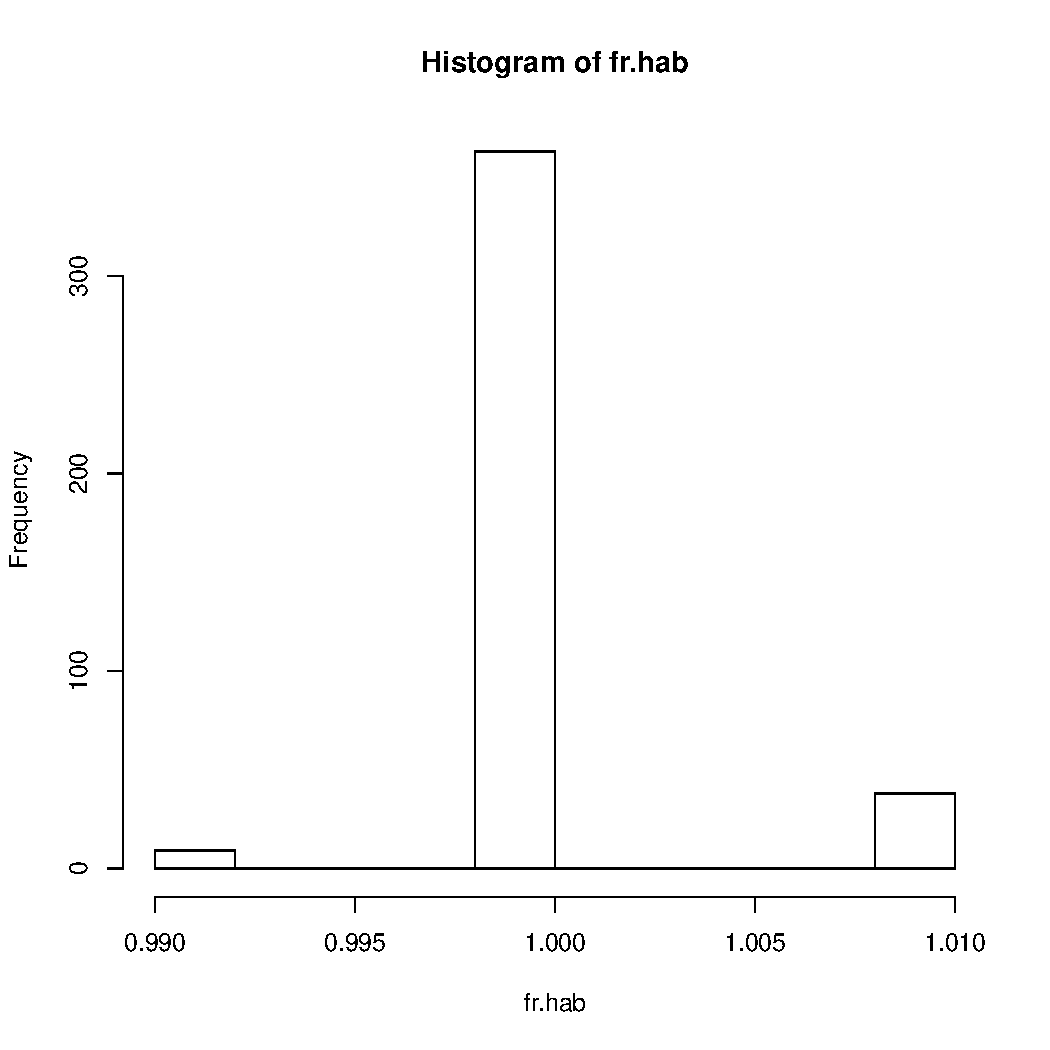
\includegraphics[width=\maxwidth]{../figures/unnamed-chunk-4-1}

\hypertarget{distribution-des-habitats}{%
\subsubsection{Distribution des
habitats}\label{distribution-des-habitats}}

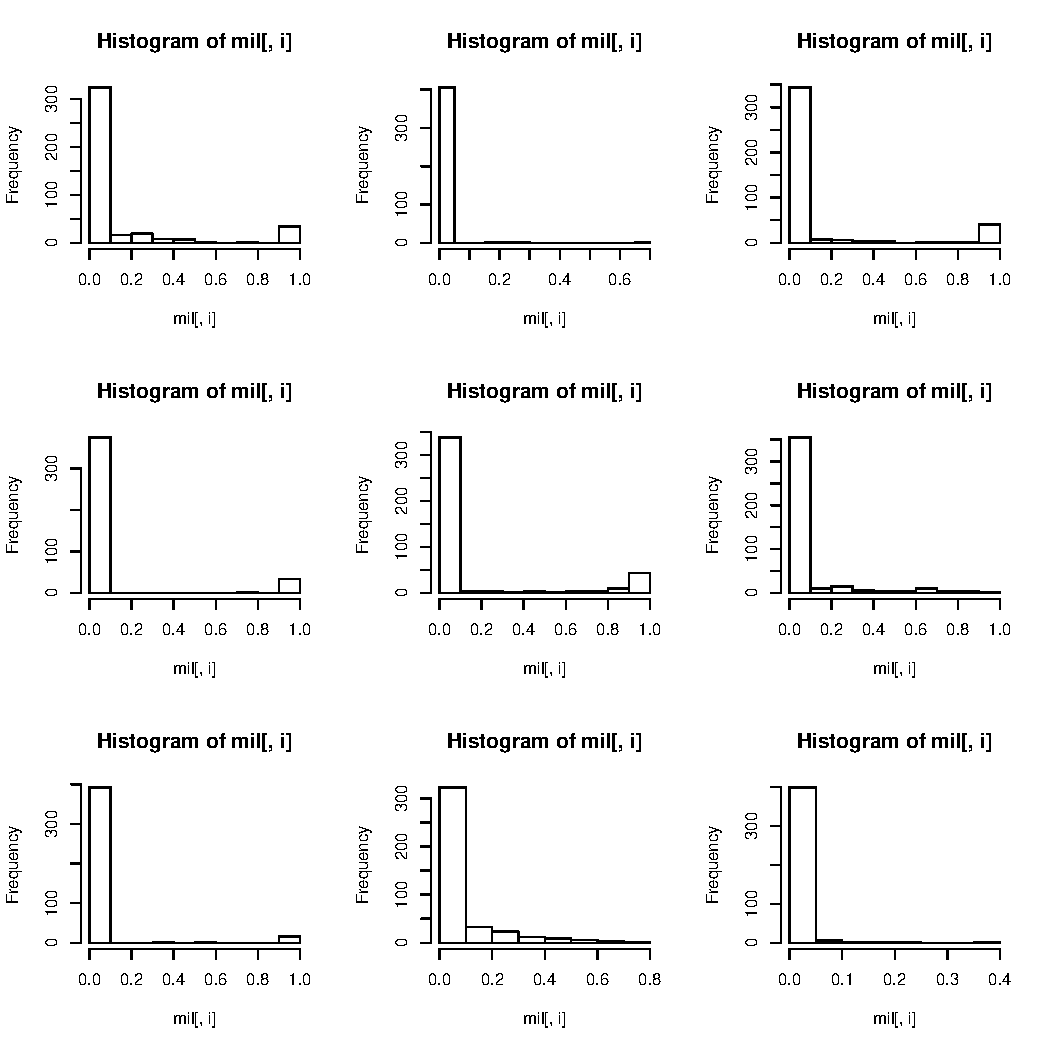
\includegraphics[width=\maxwidth]{../figures/unnamed-chunk-5-1}

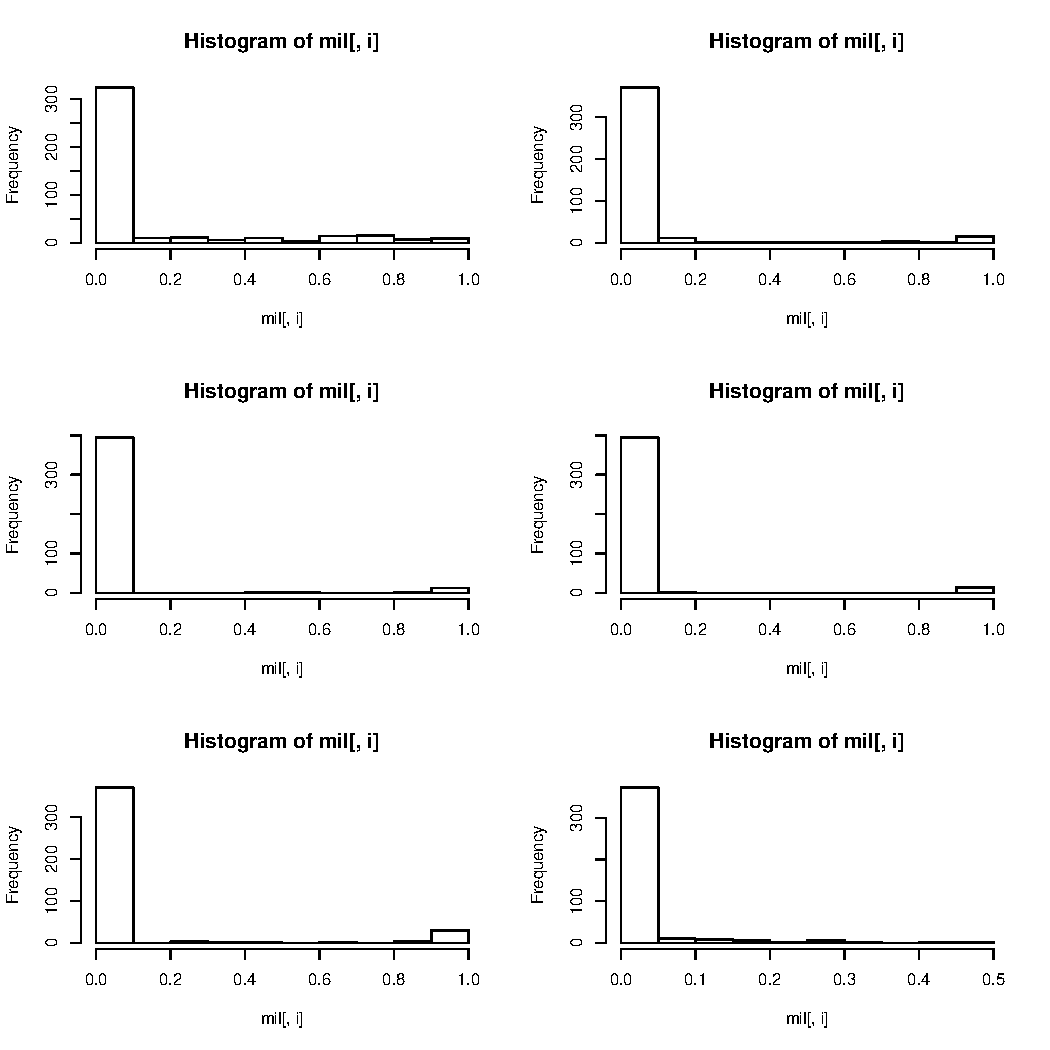
\includegraphics[width=\maxwidth]{../figures/unnamed-chunk-6-1} Les
distris des habitats posent deux problèmes :

-- la somme à 100 (en théorie)\\
-- leur asymétrie

\hypertarget{altitude}{%
\subsubsection{Altitude}\label{altitude}}

Pour l'altitude, variation assez classique :

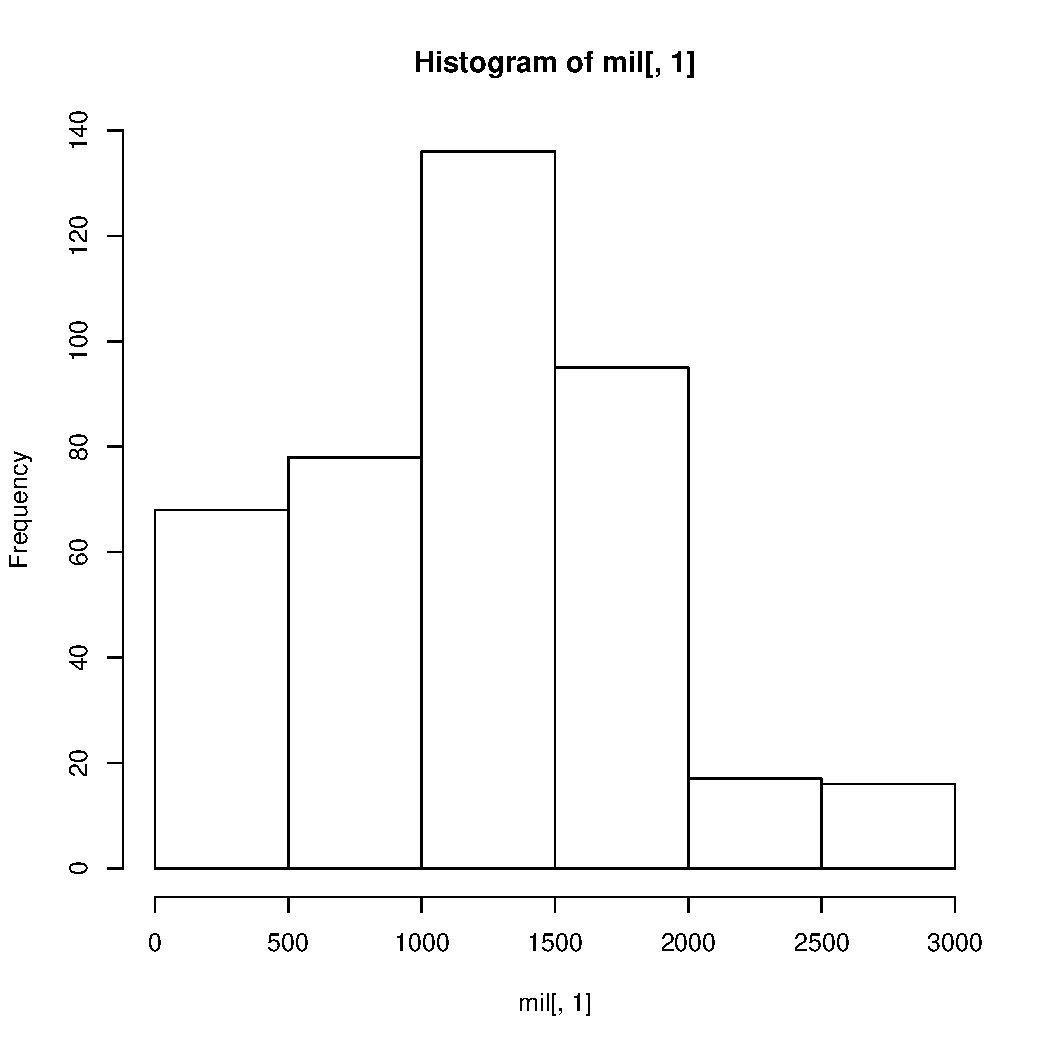
\includegraphics[width=\maxwidth]{../figures/unnamed-chunk-7-1}

\hypertarget{analyse-en-coordonnuxe9es-principales-sur-la-matrice-dhabitats}{%
\subsection{Analyse en coordonnées principales sur la matrice
d'habitats}\label{analyse-en-coordonnuxe9es-principales-sur-la-matrice-dhabitats}}

L'analyse en coordonnées principale permet de résoudre les deux
problèmes mentionnés ci dessus et d'ajouter l'altitude aux variables
d'habitat.

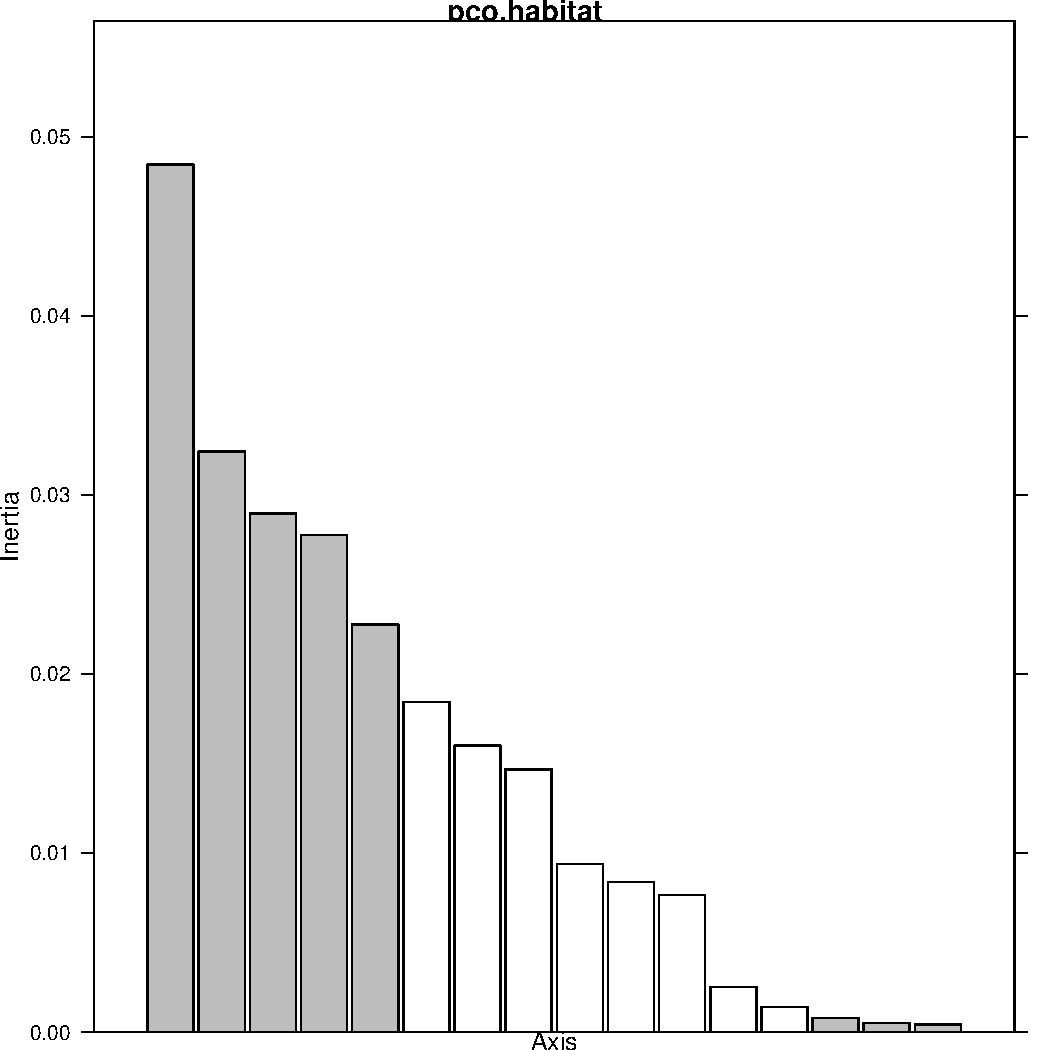
\includegraphics[width=\maxwidth]{../figures/wat-1}

\begin{verbatim}
##  [1]  20.14260  33.63155  45.67581  57.21639  66.67637  74.33942  80.98807  87.08968  90.99293  94.47521  97.65528  98.70365  99.28549  99.61633
## [15]  99.82905 100.00000
\end{verbatim}

On est sur des \% de variance expliquée assez classiques pour ce genre
de données. En première intention je retiens 5 composantes.

\hypertarget{projection-des-points-et-des-variables-axe-1-vs-chacun-des-4-autres}{%
\subsubsection{Projection des points et des variables (axe 1 vs chacun
des 4
autres)}\label{projection-des-points-et-des-variables-axe-1-vs-chacun-des-4-autres}}

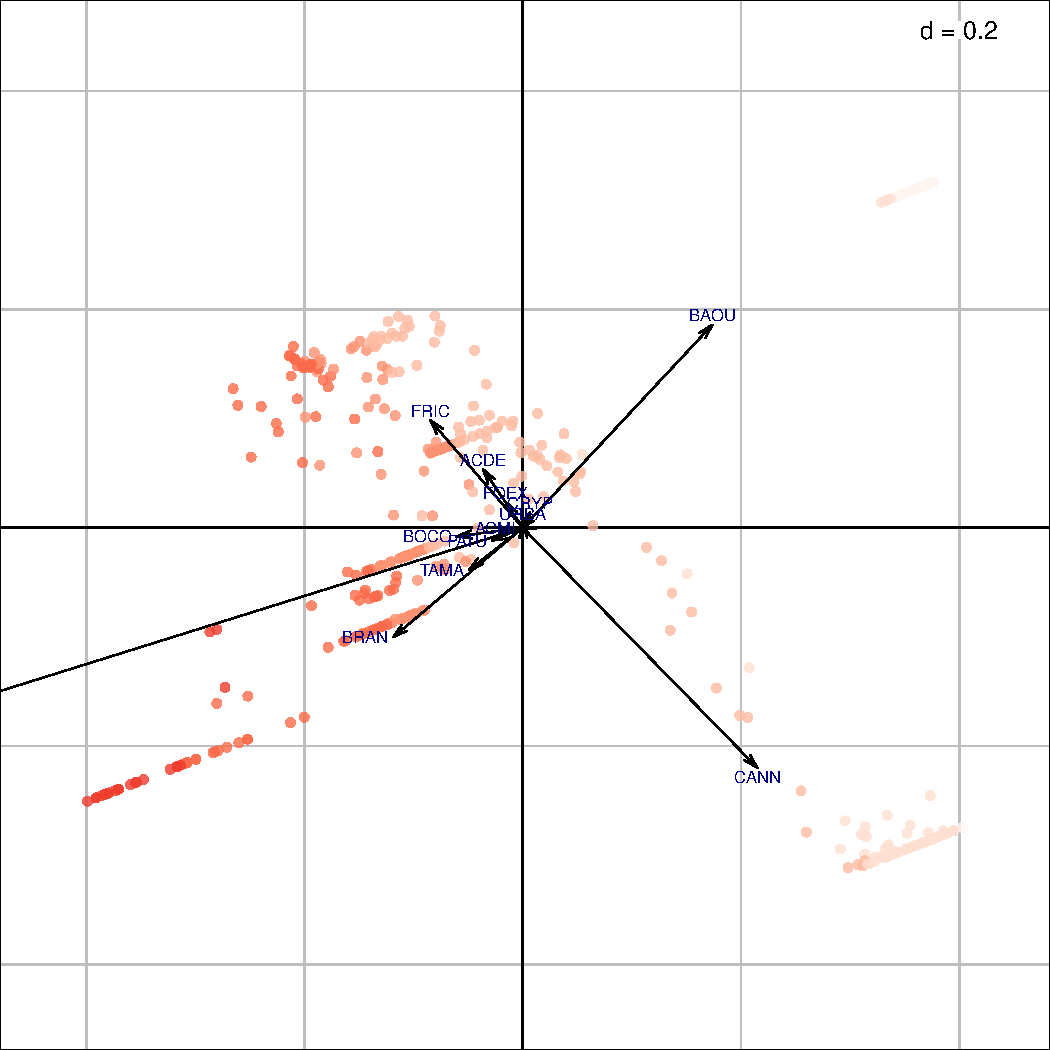
\includegraphics[width=\maxwidth]{../figures/unnamed-chunk-11-1}

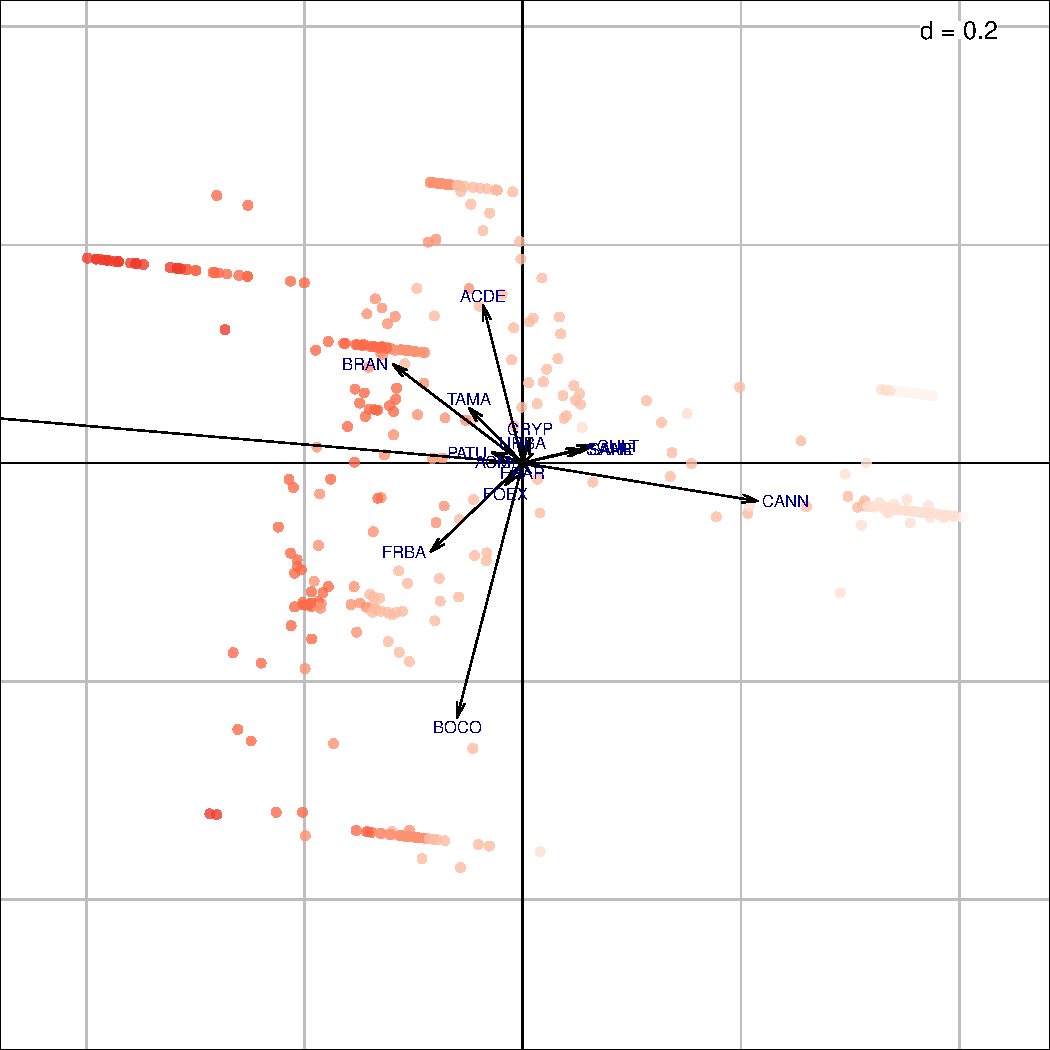
\includegraphics[width=\maxwidth]{../figures/unnamed-chunk-12-1}

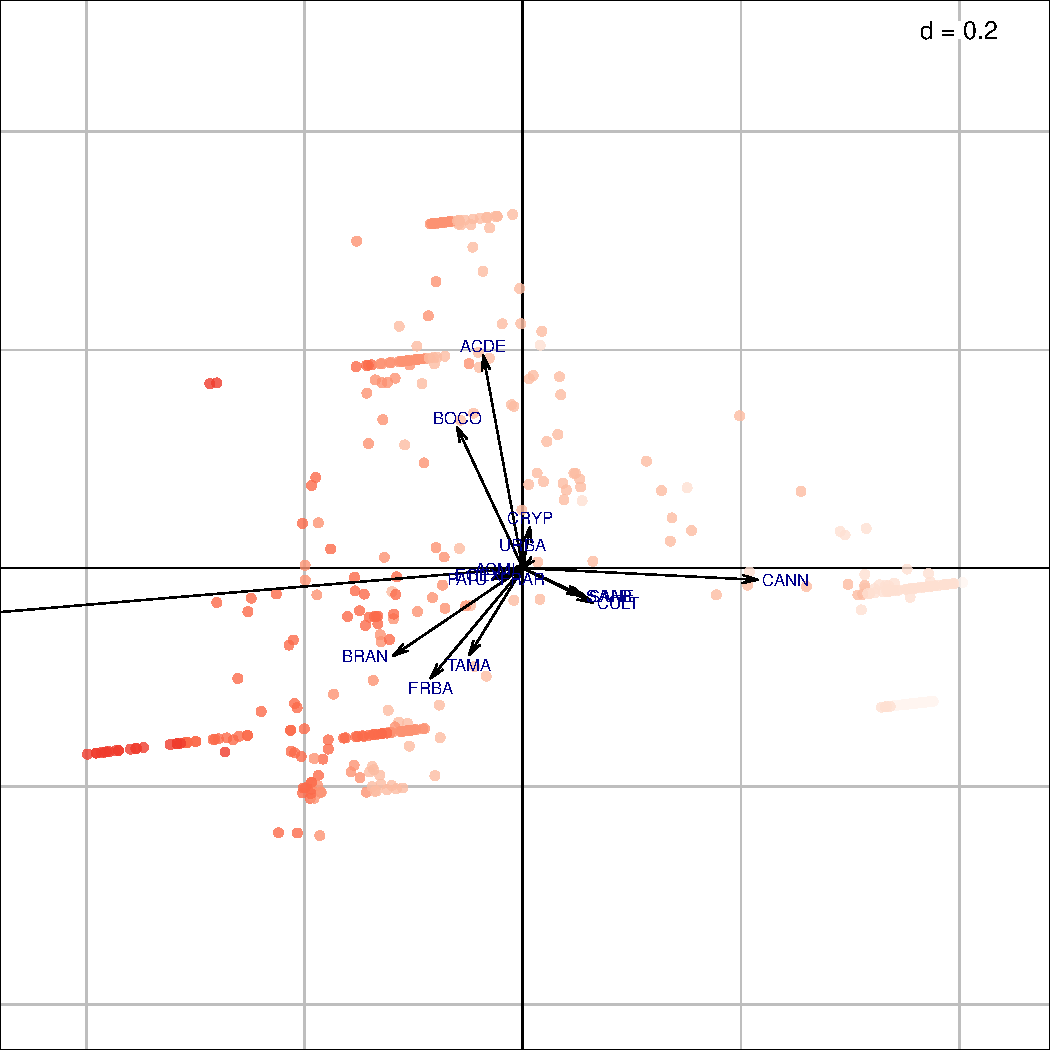
\includegraphics[width=\maxwidth]{../figures/unnamed-chunk-13-1}

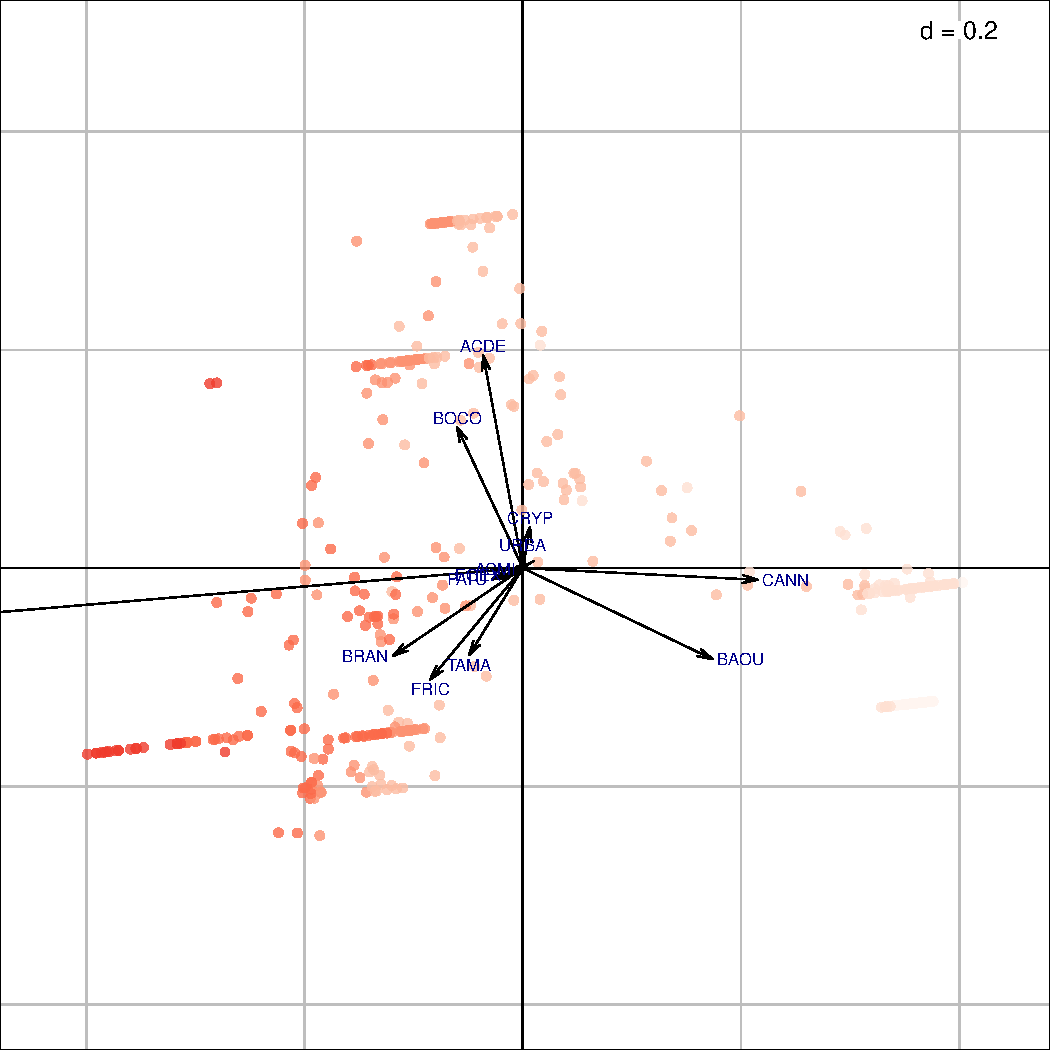
\includegraphics[width=\maxwidth]{../figures/unnamed-chunk-14-1}

\hypertarget{interpruxe9tation}{%
\subsubsection{Interprétation}\label{interpruxe9tation}}

Difficile sans bien connaître le contexte. Olivier, peux-tu avoir un
apport là dessus? Voilà ce que j'arrive à sortir:

-- PC1 = altitude -- PC2 = habitats exo vs natifs -- PC3 = ?? -- PC4 =
?? -- PC5 = ??

\hypertarget{table-oiseaux-1}{%
\subsection{table Oiseaux}\label{table-oiseaux-1}}

\hypertarget{toutes-espuxe8ces}{%
\subsubsection{Toutes espèces}\label{toutes-espuxe8ces}}

\hypertarget{afc-sur-les-abondances}{%
\paragraph{AFC sur les abondances}\label{afc-sur-les-abondances}}

\begin{verbatim}
##  [1] 0.1330918 0.2302468 0.3112237 0.3820102 0.4511414 0.5094170 0.5662222 0.6191457 0.6691835 0.7093530 0.7458145 0.7801068 0.8105675 0.8408215
## [15] 0.8685437 0.8954101 0.9199879 0.9439219 0.9661262 0.9810814 0.9929844 1.0000000
\end{verbatim}

Pas évident de retenir des gradients bien clairs, la variation est trop
graduelle. Passer en présence/absence ne change rien au problème.

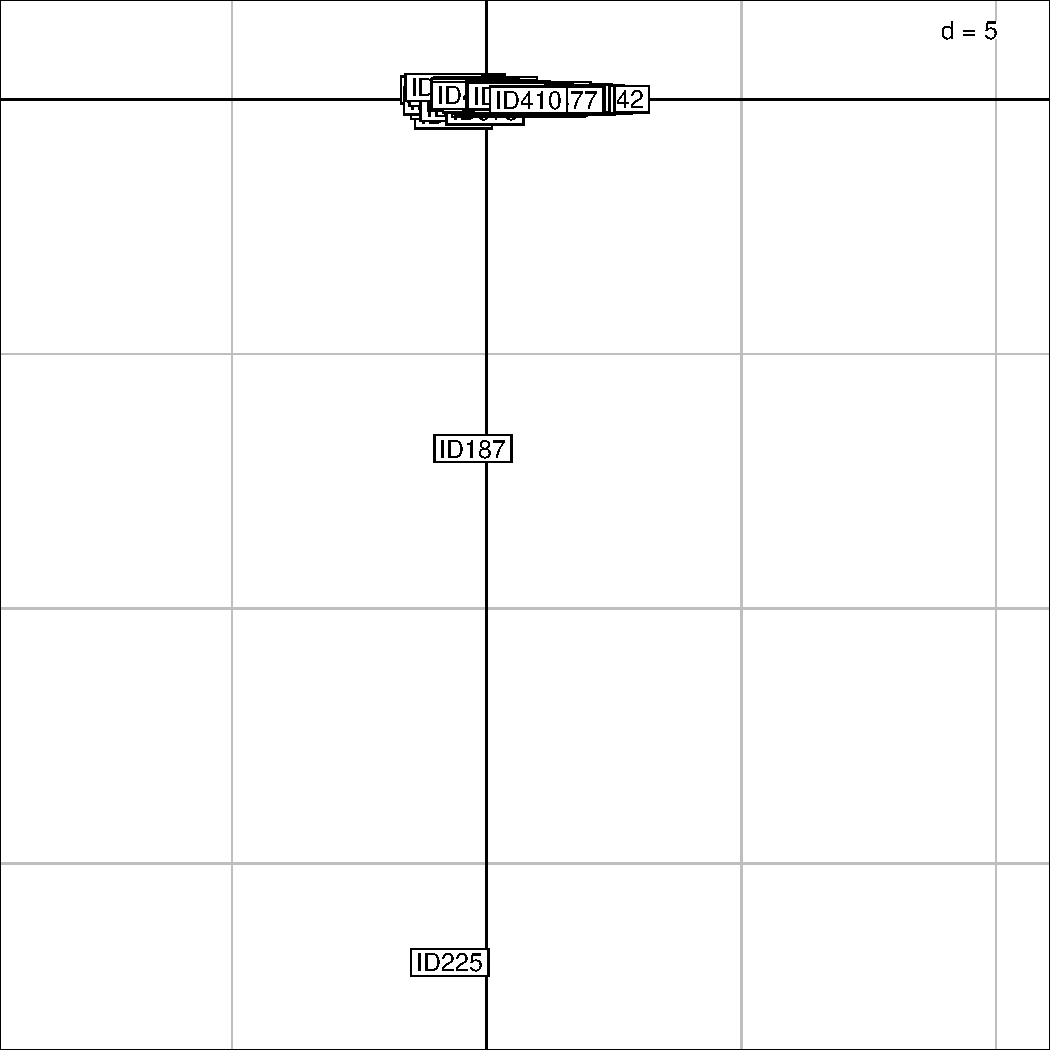
\includegraphics[width=\maxwidth]{../figures/unnamed-chunk-17-1}

Il y a deux points extrêmes :

\begin{verbatim}
##       ACTR CIMA COCH COCO COFR ESAS FOMA FRPO GEST HYBO LOPU MAMA PADO PEAS PHBO PLCU PYJO SATE STPI TEBO TUNI ZOBO ZOOL
## ID187    2    0    0    0    3    0    0    5    4    0    0    0    0    0    0    1    1    0    0    0    0    5    0
## ID225    2    0    0    0    0    0    0    3    0    0    0    0    0    0    0    0    0    0    0    0    0    0    0
\end{verbatim}

\begin{verbatim}
## ACTR CIMA COCH COCO COFR ESAS FOMA FRPO GEST HYBO LOPU MAMA PADO PEAS PHBO PLCU PYJO SATE STPI TEBO TUNI ZOBO ZOOL 
##   34    2    2    8   10   28   57    5   31    6    1    5   17   11    6   42   10   10    7    3    5   16    7
\end{verbatim}

Correspondent en particulier aux seuls points avec Francolin - voir plus
bas.

Position dans la PCOA \enquote{habitats} (tous les plans axe 1 vs l'un
des 4 autres) :

1 vs 2:

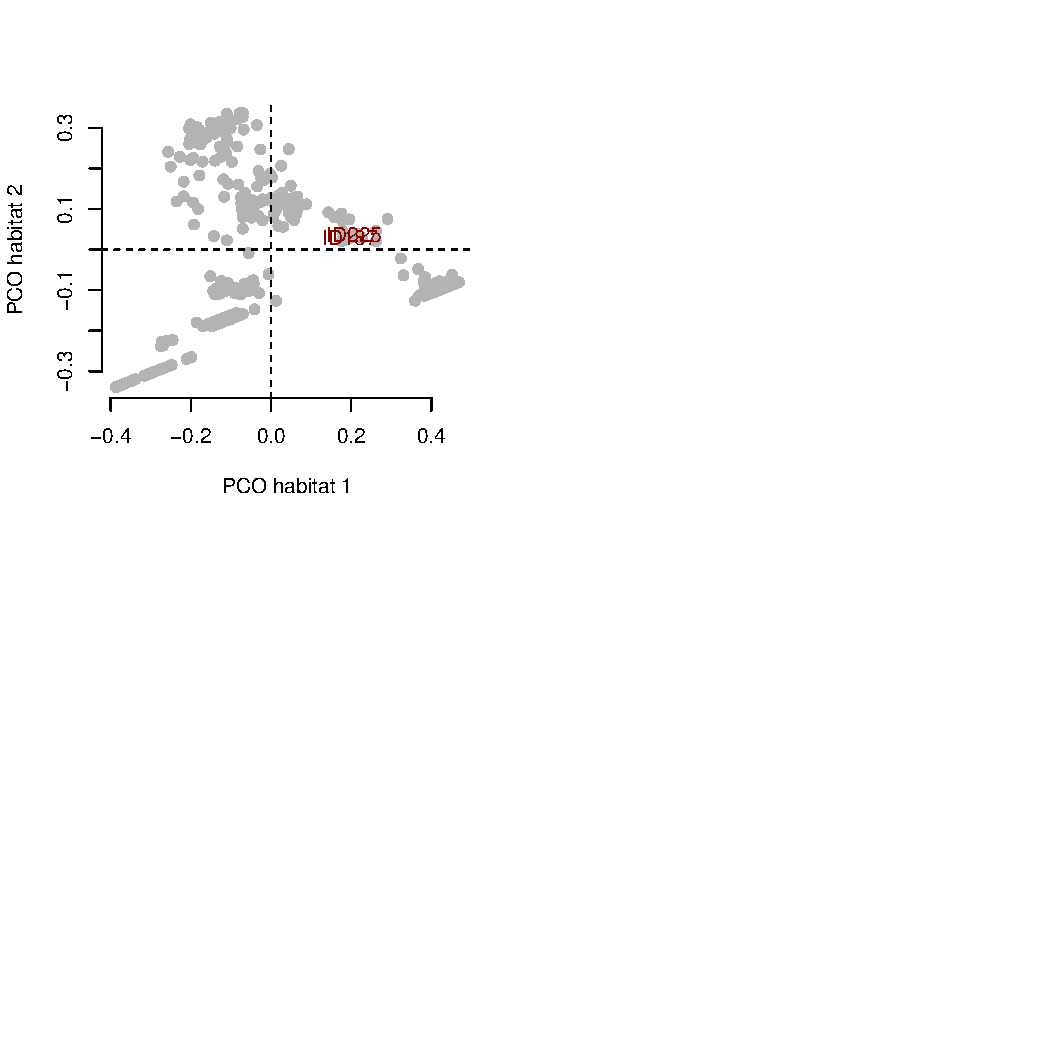
\includegraphics[width=\maxwidth]{../figures/unnamed-chunk-20-1}

1 vs 3

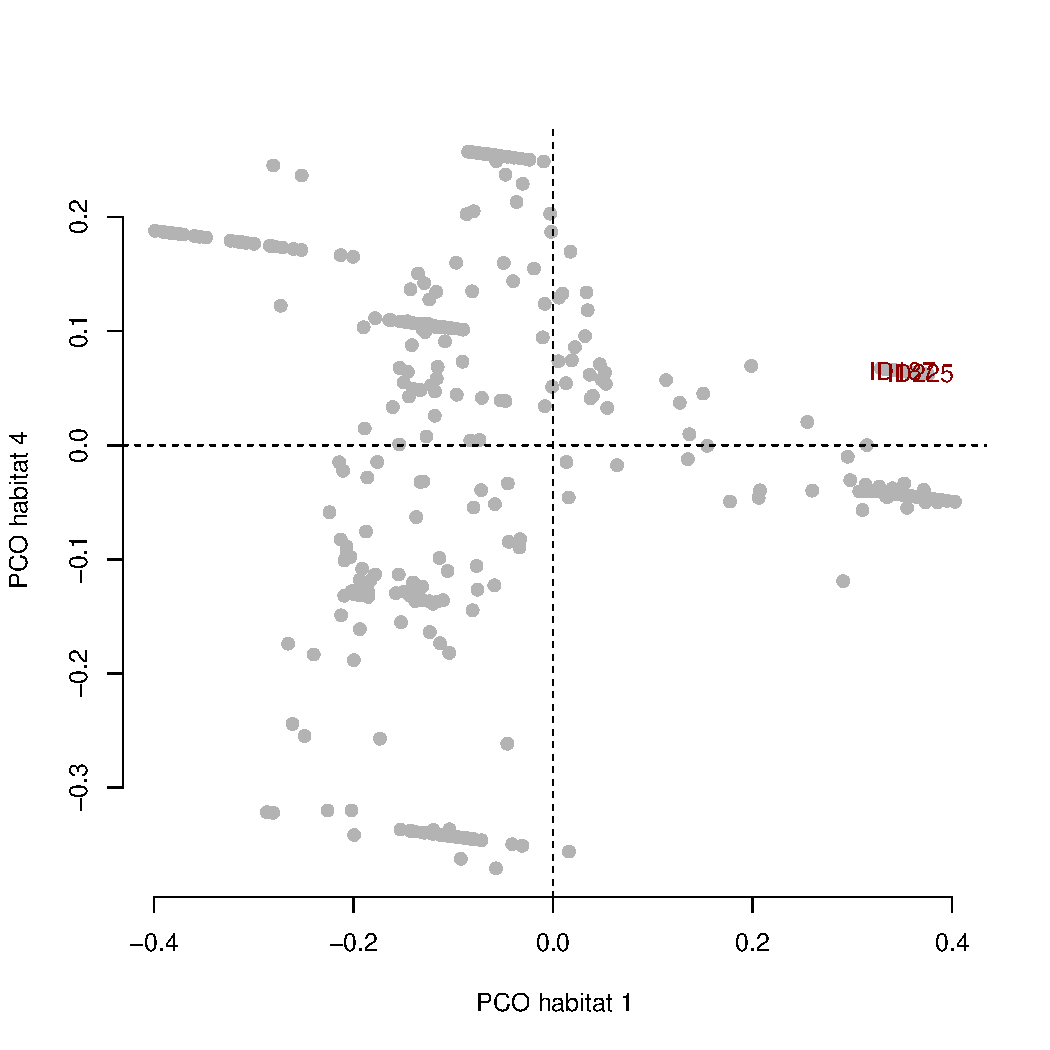
\includegraphics[width=\maxwidth]{../figures/unnamed-chunk-21-1}

1 vs 4 :

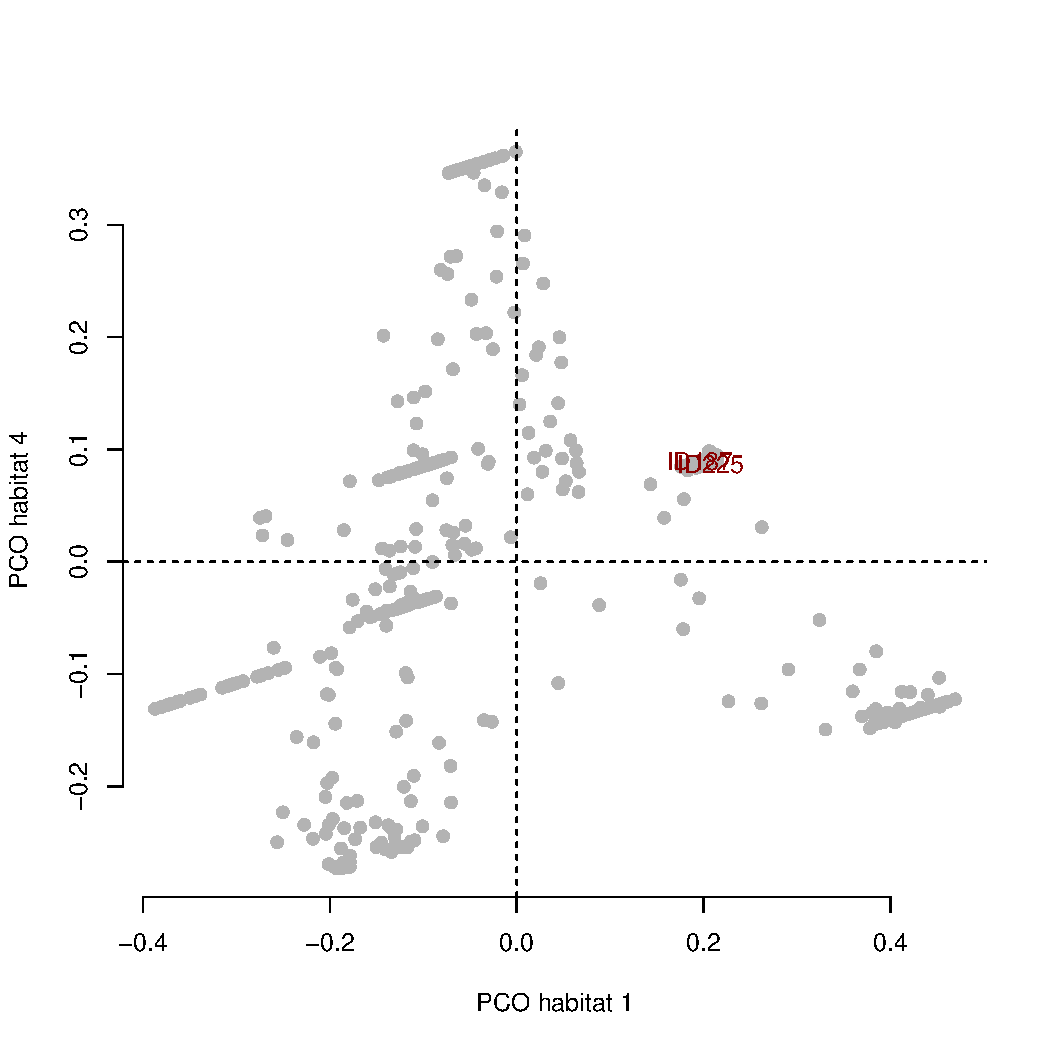
\includegraphics[width=\maxwidth]{../figures/unnamed-chunk-22-1}

1 vs 5:

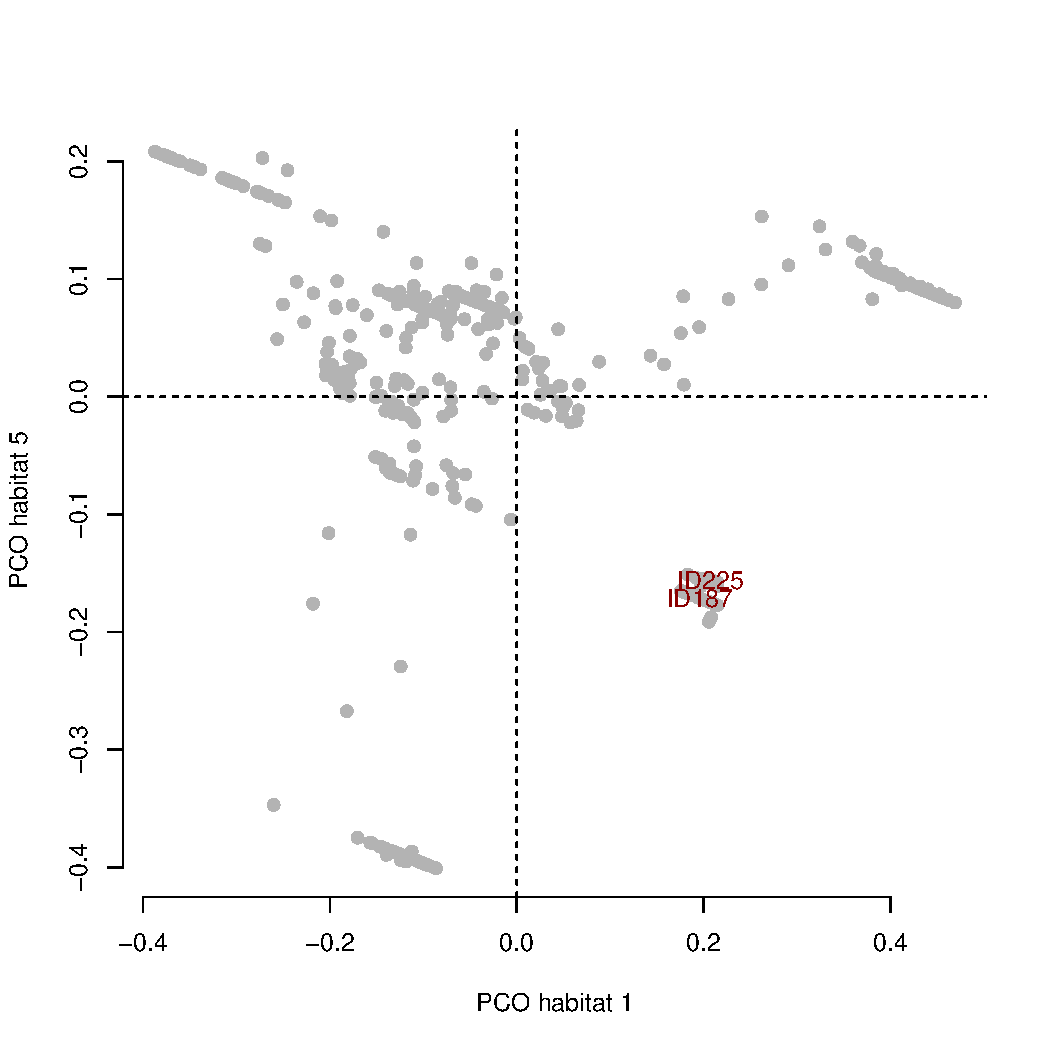
\includegraphics[width=\maxwidth]{../figures/unnamed-chunk-23-1}

L'analyse est écrasée par deux points qui n'ont rien de spécifique si ce
n'est une espèce qui leur est unique, mais leur position sur les
gradients d'habitat n'a rien d'extraordinaire. Je tente une analyse que
sur les espèces bien distribuées pour y voir plus clair.

\hypertarget{table-oiseaux-restreint-aux-espuxe8ces-pruxe9sentes-sur-5-des-points}{%
\subsection{table oiseaux : restreint aux espèces présentes sur
\textgreater{}5\% des
points}\label{table-oiseaux-restreint-aux-espuxe8ces-pruxe9sentes-sur-5-des-points}}

\hypertarget{afc-oiseaux-sans-espuxe8ces-sous-repruxe9sentuxe9es}{%
\subsubsection{AFC oiseaux sans espèces
sous-représentées}\label{afc-oiseaux-sans-espuxe8ces-sous-repruxe9sentuxe9es}}

\begin{verbatim}
## [1] 6529
\end{verbatim}

\begin{verbatim}
## [1] 326.45
\end{verbatim}

\begin{verbatim}
## [1] 65.29
\end{verbatim}

\begin{verbatim}
##        CIMA        COCH        FRPO        LOPU        MAMA        PHBO 
## 0.026829268 0.004878049 0.019512195 0.002439024 0.026829268 0.021951220
\end{verbatim}

\hypertarget{afc-sans-les-espuxe8ces-vues-sur-moins-de-5-des-points}{%
\section{AFC sans les espèces vues sur moins de 5\% des
points}\label{afc-sans-les-espuxe8ces-vues-sur-moins-de-5-des-points}}

\begin{verbatim}
##  [1] 0.1685298 0.2707443 0.3599813 0.4456636 0.5192498 0.5897839 0.6562875 0.7063508 0.7519071 0.7955382 0.8342180 0.8718459 0.9068289 0.9407699
## [15] 0.9718166 1.0000000
\end{verbatim}

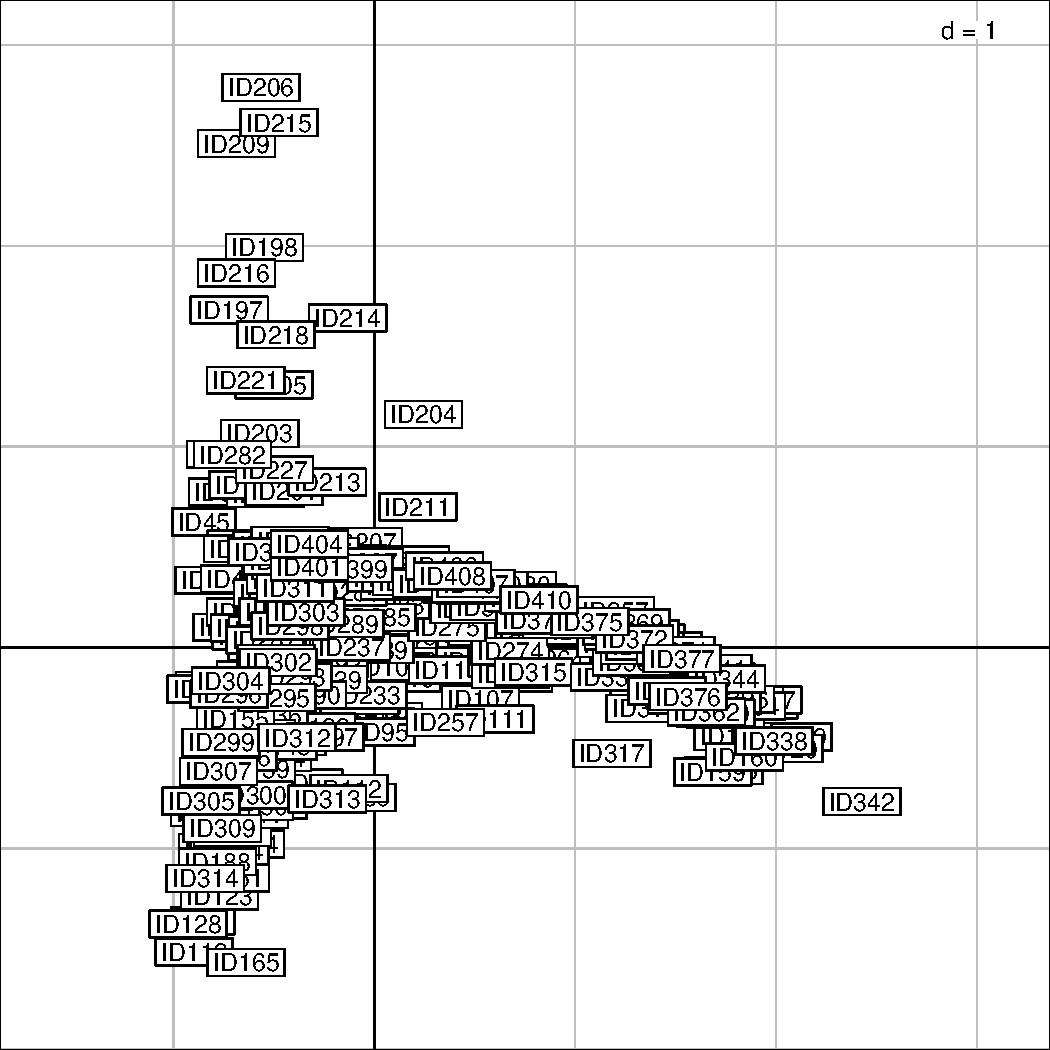
\includegraphics[width=\maxwidth]{../figures/unnamed-chunk-25-1}
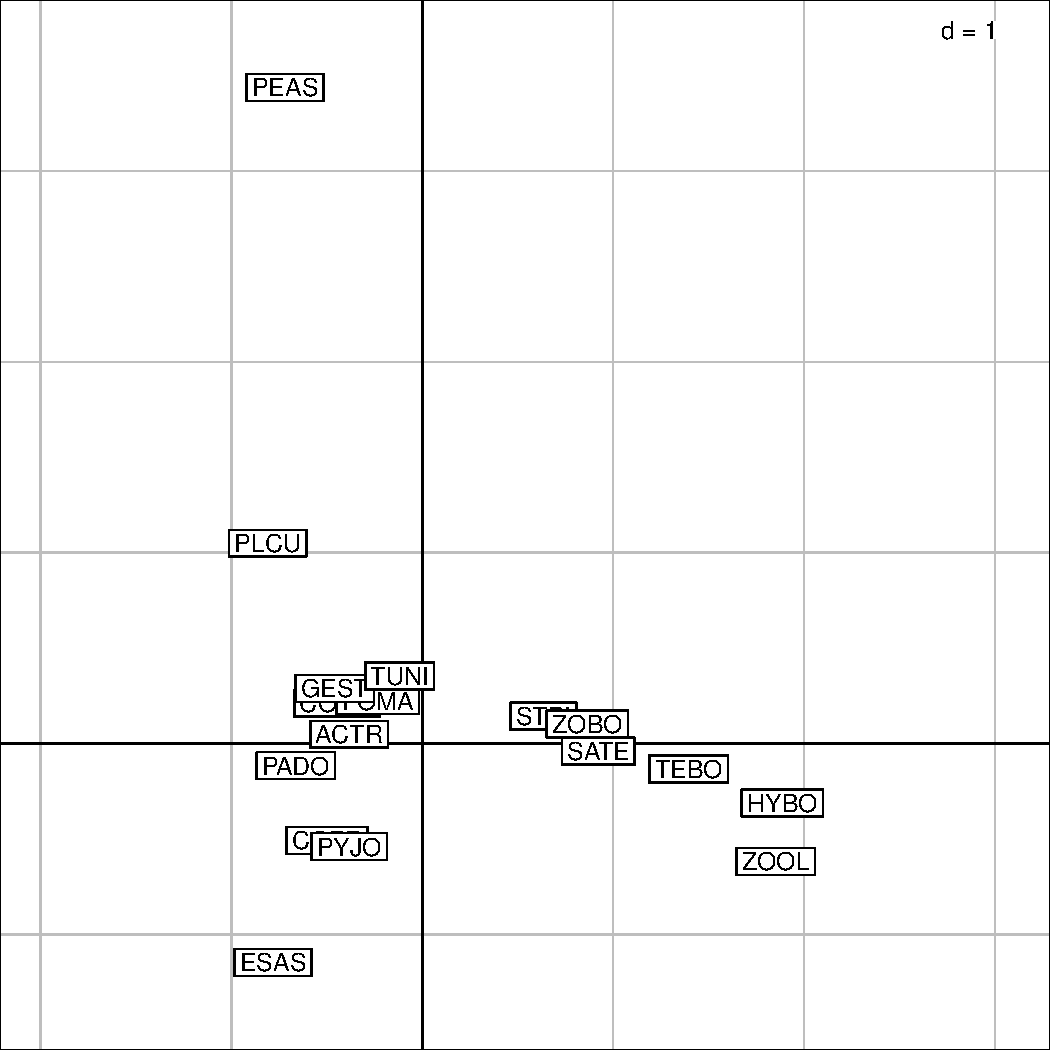
\includegraphics[width=\maxwidth]{../figures/unnamed-chunk-25-2}

Il y a un effet arche assez fort, mais au moins les points sont bien
étalés dans l'ordination

\hypertarget{analyse-fonctionnelle}{%
\section{Analyse fonctionnelle}\label{analyse-fonctionnelle}}

Cette analyse fonctionnelle ne porte \textbf{que sur l'altitude} et sur
\textbf{les abondances d'espèces log-transformées}. C'est donc très
préliminaire, mais l'altitude étant très structurante ça donne déjà une
première idée des distributions d'espèces.

\hypertarget{base-optimale}{%
\subsection{base optimale}\label{base-optimale}}

Le choix de la base fonctionnelle optimale se fait par une comparaison
entre des écarts fonctions-données pour différentes bases. Le but est
d'avoir un compromis entre sur- et sous-lissage.

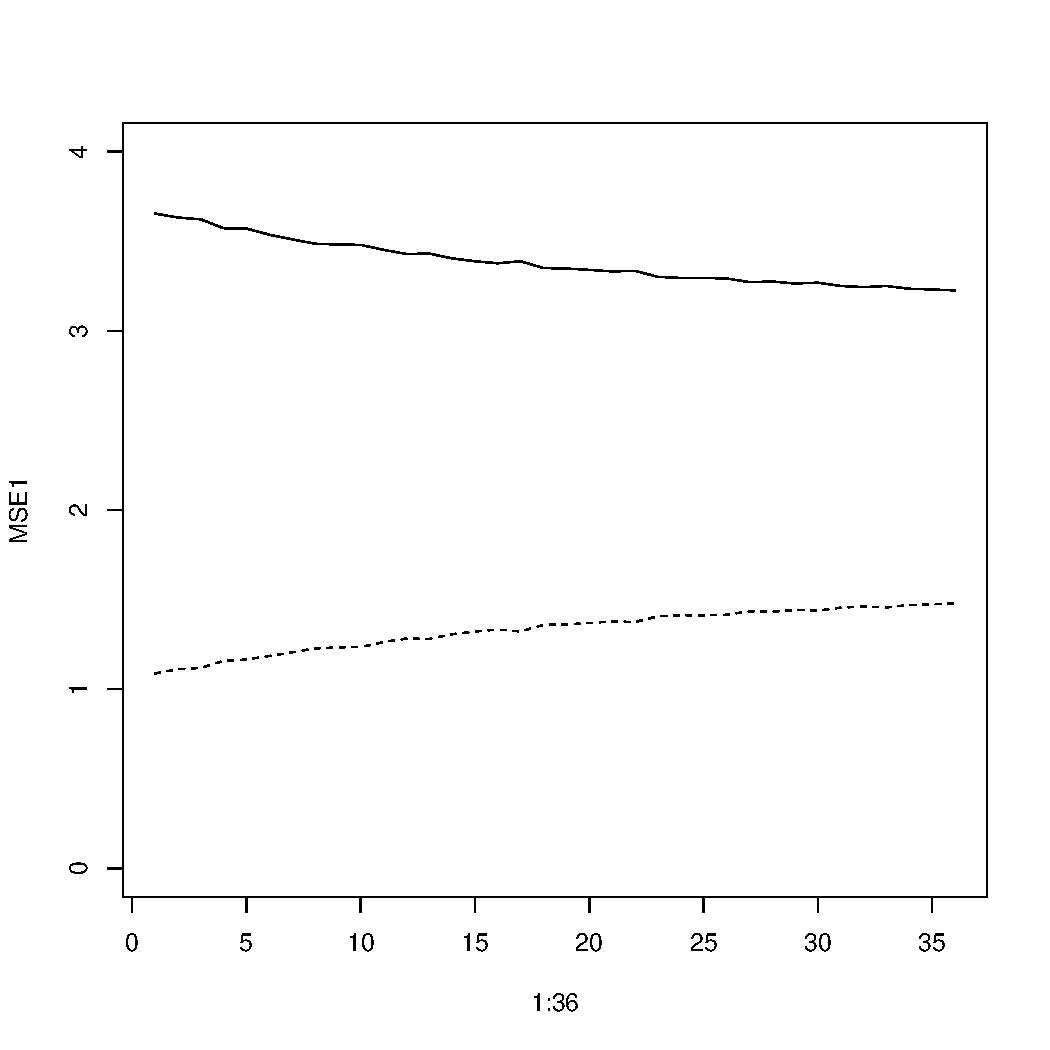
\includegraphics[width=\maxwidth]{../figures/unnamed-chunk-28-1}

Quelle que soit la base, la représentation n'est de toute façon pas très
bonne, probablement à cause des patterns de réponse à l'altitude mal
marqués (gros pics en plein milieu du gradient qui ne sont pas
modélisables facilement et / ou grosse dominance de 0 partout). Faute de
mieux on reste sur une base 4 (classique, permet de marquer 1 ou 2
optimums mais sans surlisser).

\hypertarget{analyse-fonctionnelle-1}{%
\subsection{Analyse fonctionnelle}\label{analyse-fonctionnelle-1}}

On travaille sur abondances log transformées. Les abondances et les
altitudes sont normalisées pour limiter l'impact de la rareté des
espèces et faciliter l'estimation numérique.

\hypertarget{estimation-des-courbes}{%
\subsubsection{Estimation des courbes}\label{estimation-des-courbes}}

Ces courbes décrivent, pour chaque espèce, la réponse à l'altitude
estimée à partir de splines de base 4.

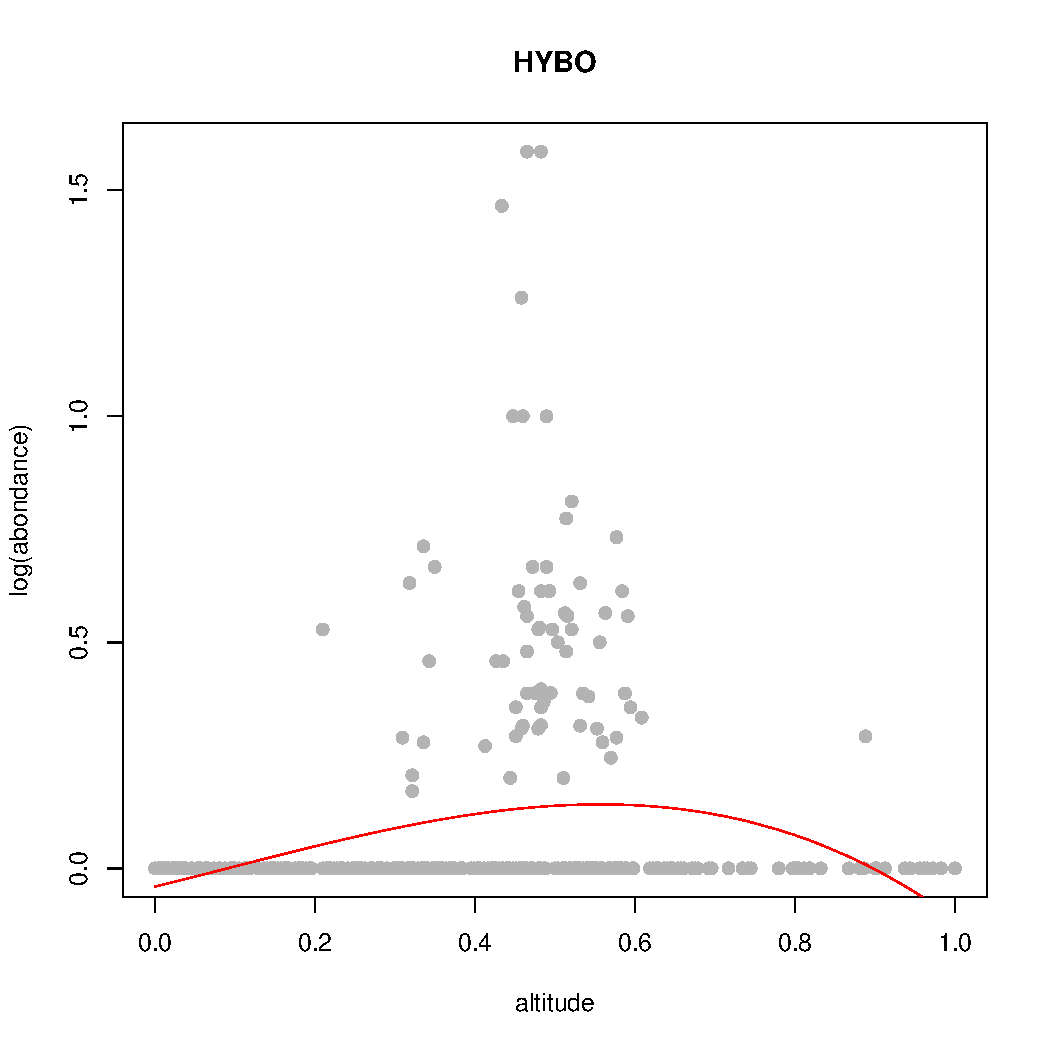
\includegraphics[width=\maxwidth]{../figures/unnamed-chunk-31-1}

La dispersion des points est toujours forte et il y a souvent des gros
pics d'abondance en milieu de gradient qui sont mal modélisables. En
général les optimums sont au bon endroit sur l'axe des altitudes mais
leur amplitude n'est pas bonne.

Comparaison des courbes de toutes les espèces :

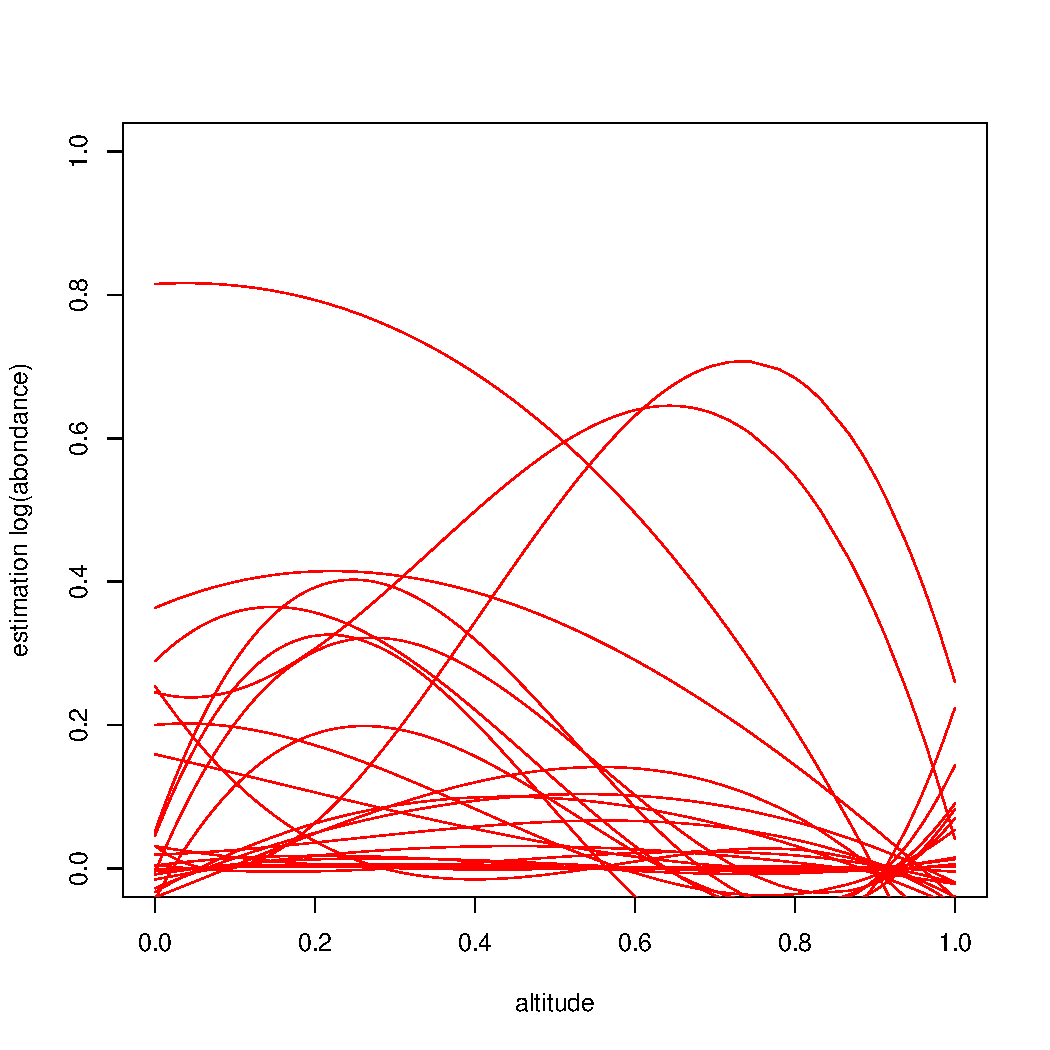
\includegraphics[width=\maxwidth]{../figures/unnamed-chunk-32-1}

\hypertarget{acp-fonctionnelle}{%
\subsection{ACP fonctionnelle}\label{acp-fonctionnelle}}

Cette ACP permet de créer des typologies de courbes. Les axes opposent
des courbes de formes différentes.

Variance expliquée :

\begin{verbatim}
## [1] 87.45767 11.89144
\end{verbatim}

\hypertarget{interpruxe9tation-des-axes}{%
\subsubsection{Interprétation des
axes}\label{interpruxe9tation-des-axes}}

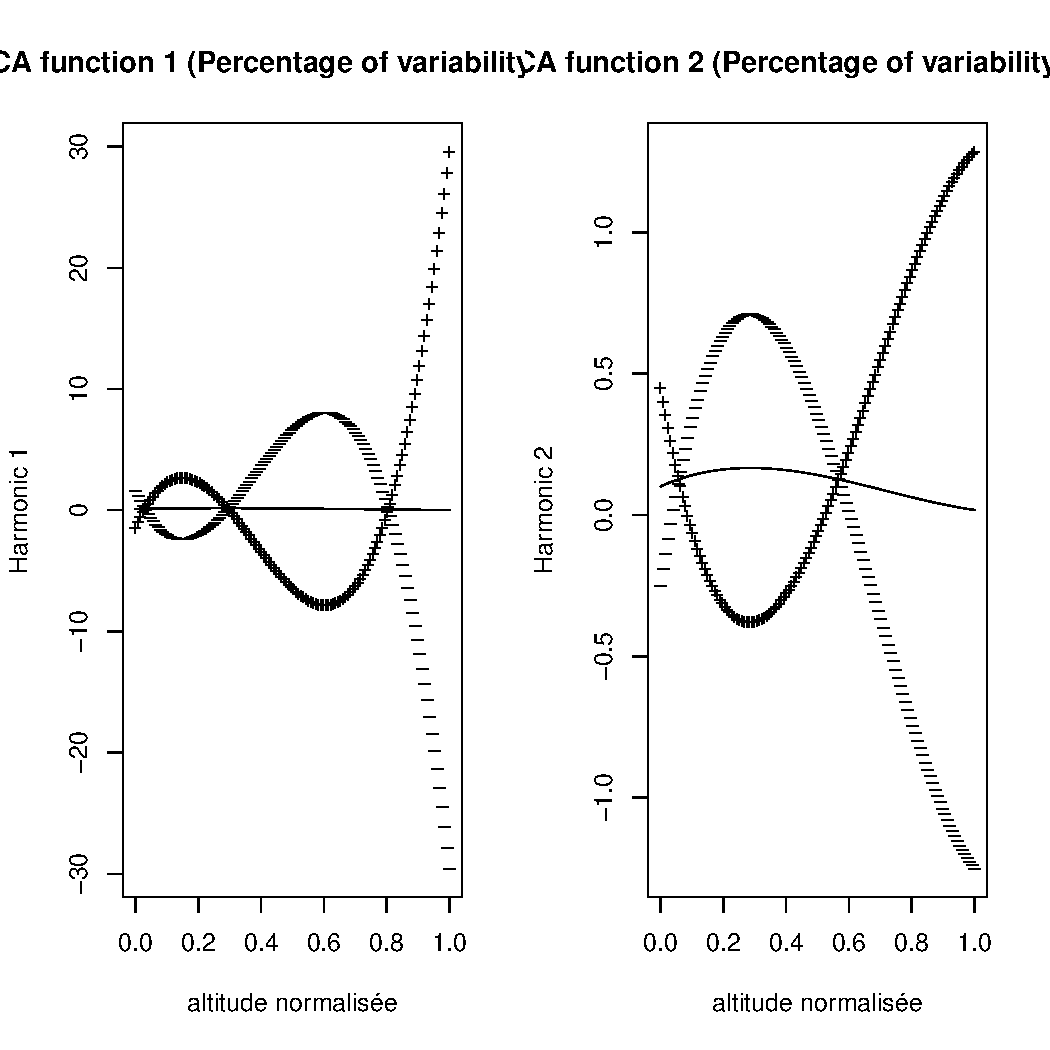
\includegraphics[width=\maxwidth]{../figures/unnamed-chunk-35-1}

La courbe en trait plein est la courbe moyenne (ici plate : en moyenne
les espèces ne répondent pas à l'altitude). La courbe \enquote{--} est
la déformation de cette courbe moyenne vers le négatif de l'axe d'ACP,
et la courbe \enquote{++} est la déformation vers les positifs.

-- \textbf{axe 1} (courbe de gauche): sépare des espèces qui diminuent
avec l'altitude (-) ou augmentent avec l'altitude (+)\\
-- \textbf{axe 2} (courbe de droite) : sépare des espèces qui ont un pic
d'abondance (-) ou un déficit d'abondance (+) dans les plaines.

Cette interprétation manque de netteté, probablement parce que les
réponses à l'altitude sont un peu anarchiques et mal définies. Il faudra
probablement réitérer l'exercice sur les axes de PCOA si on les comprend
bien. On peut aussi interpréter les axes à partir des courbes quantiles,
afin d'affiner la compréhension:

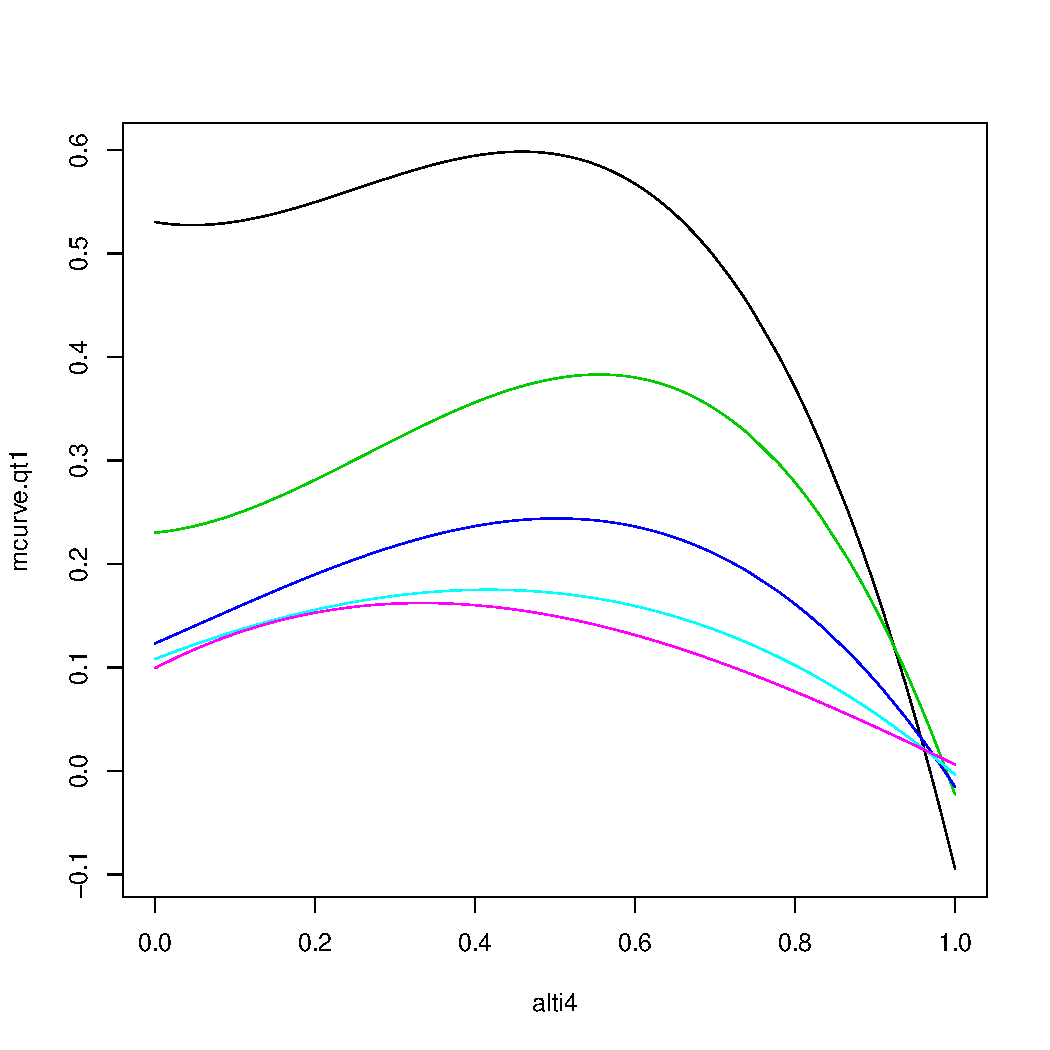
\includegraphics[width=\maxwidth]{../figures/unnamed-chunk-36-1}

Les quantiles vont du noir (-) au violet (+) et montrent bien une
typologie de patrons de réponse allant d'espèces présentes sur tout le
gradient altitudinal jusqu'à un seuil après lequel elles déclinent
brusquement à des espèces qui ont un optimum d'altitude mais une
variation peu marquée. C'est déjà plus interprétable que les
déformations.

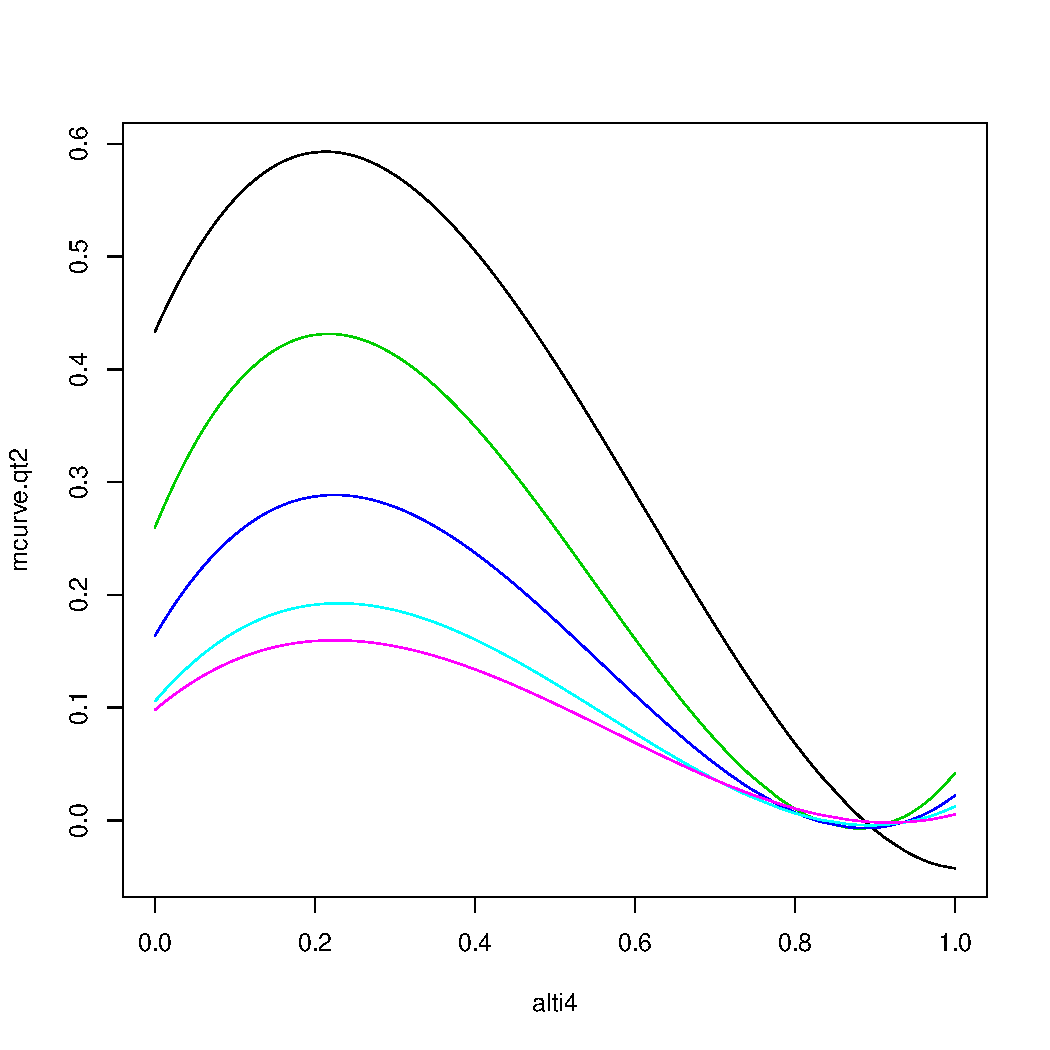
\includegraphics[width=\maxwidth]{../figures/unnamed-chunk-37-1}

Le deuxième axe semble séparer les espèces en termes de fréquence,
toutes devenant plus rares en altitude.

Le nuage de points de cette ACP:

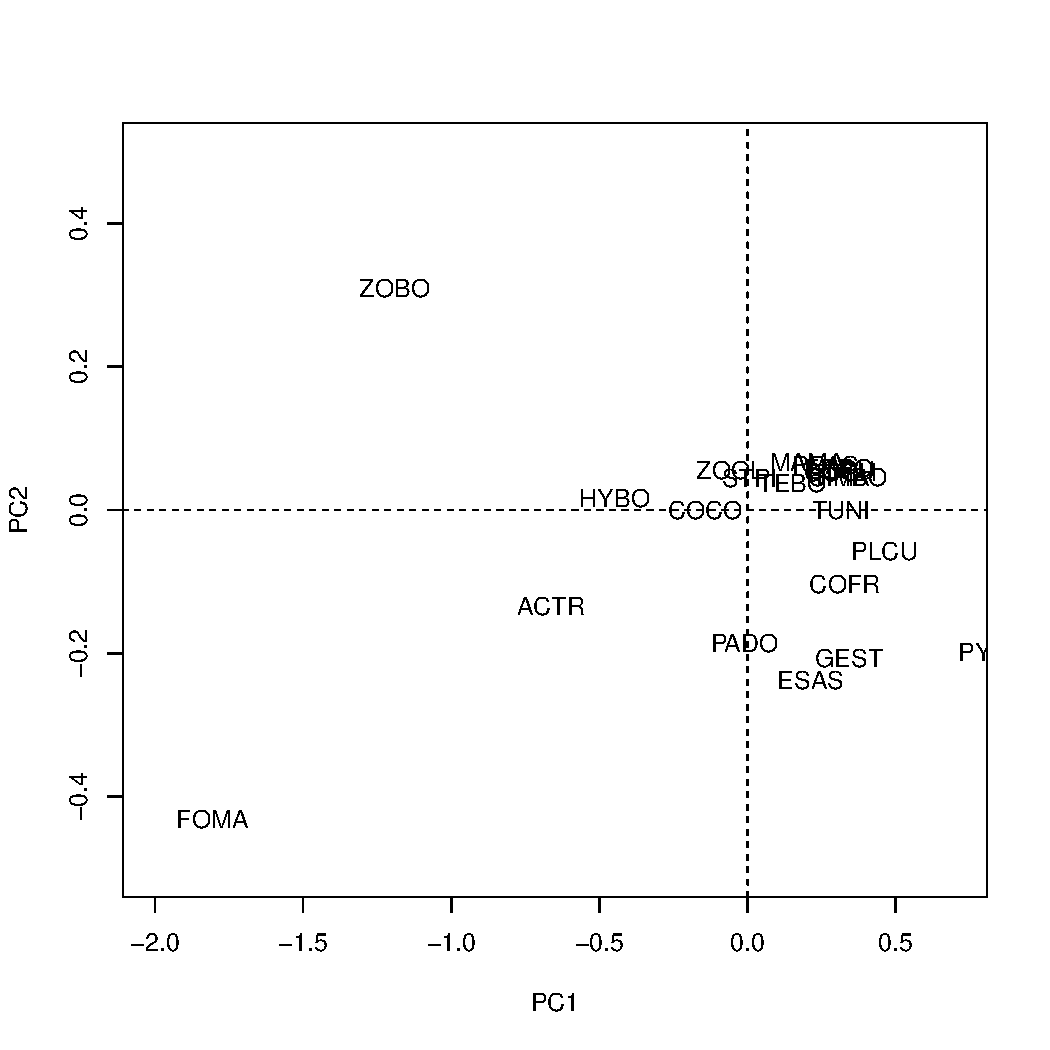
\includegraphics[width=\maxwidth]{../figures/unnamed-chunk-38-1}

La plupart des espèces est décalée dans le positif de l'axe 1, soit une
réponse assez graduelle (et faible) à l'altitude avec une baisse
d'abondance vers les sommets. Le négatif est dominé par le Foudi et le
zosterops des Mascareignes, deux espèces qui sont donc présentes sur une
bonne partie du gradient altitudinal avant une chute d'effectifs en
haute altitude. On peut le vérifier sur les courbes individuelles
(Zosterops : rouge ; Foudi : noir) :

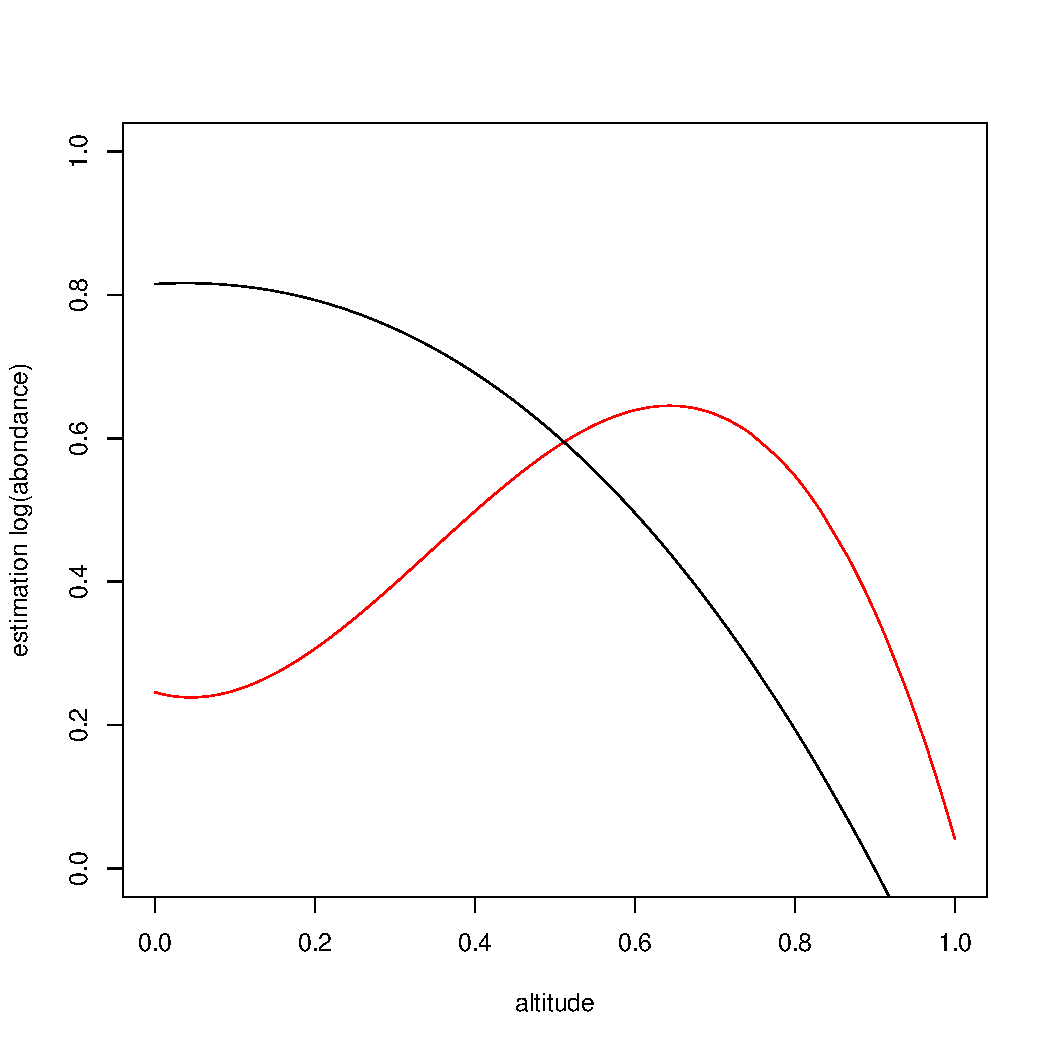
\includegraphics[width=\maxwidth]{../figures/unnamed-chunk-39-1}

\hypertarget{conclusions}{%
\section{Conclusions}\label{conclusions}}

-- L'approche à choisir : une approche statique (type PCOA / coinertie /
RLQ) ou une approche par gradient (type FDA). Dépend d'à quel point on a
confiance en l'une ou l'autre. Je n'estime pas avoir une connaissance
suffisante de l'avifaune réunionnaise pour y répondre clairement :
Olivier, ton retour serait vraiment utile.

-- la suite des analyses : là on décrit juste l'organisation des espèces
le long des gradients, il faut aller plus loin. Il y a l'approche traits
qui est facile à ajouter aux deux types d'analyses, une répartition des
ordinations sur la phylogénie, etc : à voir ce qui est le plus
intéressant à vos yeux

-- la robustesse : les éboulis de variance ne sont pas terrible, les 3-4
premiers axes des ordinations tentées ne représentent pas énormément de
variance. Ca suggère des résumés pas hyper pertinents (en tout cas
bruités) des gradients qui nous intéressent. Je suis pas très clair sur
leur représentation de la réalité du terrain (en particulier pour la
matrice habitats).

%------- bibliography ----------------




	
\end{document}
